\documentclass[12pt]{article}
%\documentclass[12pt,leqno]{article}
%% JL Cabellos at agosto 2010
\usepackage{amsmath,amssymb,amsfonts} % Typical maths resource packages
\usepackage{graphics}                 % Packages to allow inclusion
\usepackage{color}
\usepackage[spanish,english]{babel}
\usepackage{verbatim}
\usepackage{fancyvrb}
\usepackage{showkeys}
\usepackage{graphicx}
\selectlanguage{english}
%\selectlanguage{spanish}
%%%%% defs
%%%% acronimos
\def\copyr{$^\copyright$}
\def\reg{\textsuperscript{\textregistered}}
\def\tm{\textsuperscript{\texttrademark}}
\def\lufac{LUFAC${^\textsuperscript{\textregistered}}$}
%\def\depe{DP${^\textsuperscript{\texttrademark}}$}
\def\depe{DP${\texttrademark}$}
\def\ps{\mathrm{ps}}
\def\lda{\mathrm{LDA}}
\def\rpa{\mathrm{RPA}}
\def\nl{\mathrm{nl}}
\def\acu{Accu-Check\textsuperscript{\textregistered}~Performa}
\def\goni{Glucometro \'Optico No Invasivo}
\def\Reg{\textsuperscript{\textregistered}}
\def\tiniba{TINIBA\textsuperscript{\textregistered}}
\def\gw{{\it GW}}
\def\gsa{Generaci\'on del Segundo Arm\'onico}
\def\shg{Second Harmonic Generation}
\def\sfg{Sum Frequency Generation}
\def\sdf{Generaci\'on de Suma de Frecuencias}
%%%%% accent of i
\def\'#1{\if#1i{\accent19\i}\else{\accent19#1}\fi}
%%%%% compa\~nias
\def\micro{{\it Supermicro}}
%%%%% lugares
\def\lou{Laboratorio de \'Optica Ultrar\'apida}
\def\roma{Universidad de Roma II}
\def\tor{``Tor Vergata''}
\def\dti{Direcci\'on de Tecnolog\'{\i}a e Innovaci\'on}
\def\dfa{Direcci\'on de Formaci\'on Acd\'emica}
\def\dg{Direcci\'on General}
\def\da{Direcci\'on Administrativa}
\def\ifug{Insituto de F\'isica de la U. de Guanajuato}
\def\icf{Instituto de Ciencias F\'isicas}
\def\unam{Universidad Nacional Aut\'onoma de M\'exico}
\def\uguille{Universidad del Nordeste, Argentina}
\def\fotonica{Departamento de Fotonica}
\def\grupo{Propiedades \'Opticas de Nano-Sistemas, Interfases y Superficies}
\def\grupoa{PRONASIS}
%\def\grupo{Propiedades \'Opticas de Superficies e Interfases y Sistemas Nanosc\'opicos}
%\def\grupoa{POSISNA}
\def\di{Direcci\'on de Investigaci\'on}
\def\dfa{Direcci\'on de Formaci\'on Acad\'emica}
\def\cio{Centro de Investigaciones en \'Optica}
\def\ciod{Centro de Investigaciones en \'Optica, León, Guanajuato.}
\def\Conacyt{Consejo Nacional de Ciencia y Tecnolog\'ia}
\def\Concyteg{Consejo  de Ciencia y Tecnolog\'ia del Estado de Guanajuato}
\def\conacyt{CONACyT}
\def\concyteg{CONCyTEG}
\def\lagos{Centro Universitario de los Lagos}
\def\udeg{Universidad de Guadalajara}
\def\dinv{Direcci\'on de Investigaci\'on}
\def\dop{Department of Physics}
\def\uoft{University of Toronto}
\def\ua{University of Texas at Austin}
\def\icf{Instituto de Ciencias Físicas, UNAM, Cuernavaca}
%%%%% gente
%% grupo
\def\gabriel{Gabriel Ramos Ortíz}
\def\ramon{Ram\'on~ Carriles~ Jaimes}
\def\ramonm{Ram\acute{o}n~ Carriles~ Jaimes}
\def\enrique{Enrique~ Castro~ Camus}
\def\raul{Ra\'ul Alfonso V\'azquez Nava}
\def\raulm{Ra\acute{u}l~ Alfonso~ V\acute{a}zquez~ Nava}
\def\beto{Norberto~ Arzate~ Plata}
\def\bmsa{Bernardo S. Mendoza}
\def\bms{Bernardo~ Mendoza~ Santoyo}
%% alumnos
\def\cesar{C\'esar Castillo Quevedo}
\def\cabellos{Jos\'e Luis Cabellos Quiroz}
\def\tona{Tonatiuh Rangel Gordillo}
\def\temok{Juan Cuauhtemoc Salazar Gonz\'alez}
\def\adan{Luis Adan Mart\'inez Jim\'enez}
\def\sean{Sean Martin Anderson}
\def\reinaldo{Reinaldo Zapata Pe\~na}
%%% alumnos del grupo
%% enrique
%Maestria:
\def\jorgee{Jorge Alberto Caballero Mendoza}
\def\sofia{Sofía Carolina Corzo García}
\def\ruth{Ruth Julieta Medina López} 
%Doctorado: 
\def\juane{Juan Jes\'us S\'anchez S\'anchez}
%Licenciatura
\def\alma{Alma Gabriela González Patlán}
%(con Ramon): 
\def\sergioer{Sergio Augusto Romero Serv\'{\i}n}
%% Raul
%Maestria:
\def\enriquer{Enrique Arag\'on Navarro}%udg
\def\salomonr{Salom\'on Rodr\'{\i}guez Carrera}
\def\hectorr{H\'ector Santiago Hern\'andez}
\def\victor{Victor Manuel Villanueva Reyes}
%% Ramon
%Maestria:
\def\alfredora{Alfredo Campos Mej\'{\i}a}
%% Beto
%Doctorado
\def\noe{No\'e Gonz\'alez Baquedano}
%% otros
\def\liliana{Liliana Wilson Herr\'an}
\def\gerardo{Gerardo E. S\'anchez Garc\'{\i}a Rojas}
\def\amalia{Amalia Mart\'inez Garc\'{\i}a}
\def\nacho{Ing. José Ignacio Diego Manrique}
\def\tere{Teresita del Niño Jesús Pérez Hernández}
\def\elder{Elder de la Rosa Cruz}
\def\gonzalo{Gonzalo P\'aez Padilla}
\def\wlm{W. Luis Moch\'an Backal}
\def\oracio{Oracio C. Barbosa Garc\'ia}
\def\hector{H\'ector Hugo S\'anchez Hern\'andez}
\def\marco{Marco Antonio Escobar-Acevedo}
\def\gil{Alejandro Gil-Villegas Montiel}
\def\ernesto{Ernesto Carlos Cort\'es Morales}
\def\fms{Fernando Mendoza Santoyo}
\def\cuevas{Francisco Javier Cuevas de la Rosa}
\def\brenda{Brenda Esmeralda Matr\'inez Z\'erega}
\def\guille{Guillermo Ortiz}
\def\cesar{Cesar Castillo Quevedo}
\def\sipe{Prof. John Sipe}
\def\mike{Prof. Michael Downer}
\def\jems{Jorge Enrique Mej\'ia S\'anchez}
\def\lamon{Ram\'on Rodr\'iguez Vera}
\def\ldp{Luis de la Pe\~na}
\def\sole{Rodolfo Del Sole}
\def\lucia{Lucia Reining}
\def\sch{Schr\"odinger}
\def\Cuevas{Francisco J. Cuevas de la Rosa}
%%%%% categorias
\def\ita{Investigador Titular A}
\def\itb{Investigador Titular B}
\def\itc{Investigador Titular C}
\def\itd{Investigador Titular D}
\def\ite{Investigador Titular E}
\def\sr{Senior Researcher}
\def\iac{Investigador Asociado C}    
\def\alm{Alumno de Maestr\'ia}
\def\ald{Alumno de Doctorado}
\def\all{Alumno de Licenciatura}
\def\adei{Asistente de Investigaci\'on}
\def\sniIII{S.N.I. nivel III}
\def\sni{S.N.I.}
\def\cv{Currículum Vitae}
%%%%%% fonts
\def\tit{\sf}
\def\col{\sc}
\def\alu{\it} % for students
\def\cual{2$^{do}$}
\def\anno{2005}
\def\spe{\vspace{.12cm}}
%%%%%% cosas
\def\capa{capa-a-capa}
\def\espin{espintr\'onica}
\def\oespin{optoespintr\'onica}
\def\proyecto{Photon Assisted Spintronics}
\def\npro{48915}
\def\cvk{cv\mathbf{k}}
\def\cvkp{c'v'\mathbf{k}'}
%%%%%% revistas
\def\prb{Physical Review B}
\def\prl{Physical Review Letters}
\def\ol{Optics Letters}
\def\opn{Optics and Photonics News}
\def\pssc{physica status solidi (c)}
%%%%%%%%%%%%%%%%%%%%%%%%%%%%%%%%%%%%%%%
%%%%%% griegas
\def\ga{\alpha}
\def\gb{\beta}
\def\gga{\gamma}
\def\gGa{\Gamma}
\def\go{\omega}
\def\got{\tilde\omega}
\def\gO{\Omega}
\def\gr{{\rho}}
\def\ge{\epsilon}
\def\ve{\varepsilon}
\def\gve{\varepsilon}
\def\gd{\delta}
\def\gD{\Delta}
\def\gl{\lambda}
\def\gs{\sigma}
\def\gS{\Sigma}
\def\gbs{\overline{\sigma}}
\def\gka{\kappa}
%%%%%% griegas with tilde
\def\gta{\tilde{\alpha}}
\def\gtb{\tilde{\beta}}
\def\gtga{\tilde{\gamma}}
\def\gto{\tilde{\omega}}
\def\gtO{\tilde{\Omega}}
\def\gtr{\tilde{\rho}}
\def\gte{\tilde{\epsilon}}
\def\vte{\tilde{\varepsilon}}
\def\gtd{\tilde{\delta}}
\def\gtD{\tilde{\Delta}}
\def\gtl{\tilde{\lambda}}
\def\gts{\tilde{\sigma}}
\def\gtS{\tilde{\Sigma}}
%%%%%% romans with tilde
\def\bftr{\tilde{\mathbf{r}}}
\def\bftp{\tilde{\mathbf{p}}}
\def\bftv{\tilde{\mathbf{v}}}
\def\ta{\tilde{a}}
\def\tb{\tilde{b}}
\def\tr{\tilde{r}}
\def\tp{\tilde{p}}
\def\tV{\tilde{V}}
\def\tv{\tilde{v}}
%%
\newcommand{\ham}{\hat{\mathcal H}}
%%%%%% bra kets
\newcommand{\la}{\langle}
\newcommand{\ra}{\rangle}
\newcommand{\ket}[1]{| #1 \rangle}
\newcommand{\bra}[1]{\langle #1 |}
\newcommand{\braket}[2]{\langle {#1} | {#2} \rangle}
\newcommand{\ketbra}[2]{| {#1} \rangle {#1} \langle {#2} |}
\newcommand{\ave}[1]{\langle {#1} \rangle}
\newcommand{\dotp}[2]{\mathbf{#1} \cdot \mathbf{#2}}
%%%%%% averages
\newcommand{\prom}[1]{\langle {#1} \rangle}
%%%%%% creation and annihilation operators
\newcommand{\oa}{\hat a^{\tiny\strut}}
\newcommand{\oad}{\hat a^\dagger}
\newcommand{\oadk}{\hat a^\dagger_{\mathbf k}}
\newcommand{\oak}{\hat a^{\tiny\strut}_{\mathbf k}}
\newcommand{\obd}[1]{\hat b^\dagger_{#1}}
\newcommand{\ob}[1]{\hat b^{\tiny\strut}_{#1}}
%%%%%% Caligraphic
\newcommand{\cala}{{\mathbf{\cal A}}}
\newcommand{\calb}{{\mathbf{\cal B}}}
\newcommand{\calc}{{\mathbf{\cal C}}}
\newcommand{\cald}{{\mathbf{\cal D}}}
\newcommand{\cale}{{\mathbf{\cal E}}}
\newcommand{\calf}{{\mathbf{\cal F}}}
\newcommand{\calh}{{\mathbf{\cal H}}}
\newcommand{\cali}{{\mathbf{\cal I}}}
\newcommand{\calp}{{\mathbf{\cal P}}}
\newcommand{\calg}{{\mathbf{\cal G}}}
\newcommand{\calv}{{\mathbf{\cal V}}}
\newcommand{\call}{{\cal L}}
\newcommand{\calo}{{\cal O}}
\newcommand{\caln}{{\cal N}}
\newcommand{\calr}{{\cal R}}
\newcommand{\cals}{{\cal S}}
\newcommand{\calt}{{\cal T}}
\newcommand{\calu}{{\cal U}}
\newcommand{\calw}{{\cal W}}
\newcommand{\calbd}{\boldsymbol{\mathcal{\cal D}}}
\newcommand{\calbj}{\boldsymbol{\mathcal{\cal J}}}
\newcommand{\calbp}{\boldsymbol{\mathcal{\cal P}}}
\newcommand{\calbv}{\boldsymbol{\mathcal{\cal V}}}
\newcommand{\calbs}{\boldsymbol{\mathcal{\cal S}}}
\newcommand{\calbg}{\boldsymbol{\mathcal{\cal G}}}
%%%%%% mathematicla bold roman & greek
\newcommand{\mbf}[1]{\mathbf{#1}}
\newcommand{\mbg}[1]{\boldsymbol{\mathcal {#1}}}
\newcommand{\bfA}{\mathbf{A}}
\newcommand{\bfB}{\mathbf{B}}
\newcommand{\bfC}{\mathbf{C}}
\newcommand{\bfD}{\mathbf{D}}
\newcommand{\bfE}{\mathbf{E}}
\newcommand{\bfF}{\mathbf{F}}
\newcommand{\bfG}{\mathbf{G}}
\newcommand{\bfH}{\mathbf{H}}
\newcommand{\bfI}{\mathbf{I}}
\newcommand{\bfJ}{\mathbf{J}}
\newcommand{\bfK}{\mathbf{K}}
\newcommand{\bfL}{\mathbf{L}}
\newcommand{\bfM}{\mathbf{M}}
\newcommand{\bfN}{\mathbf{N}}
\newcommand{\bfP}{\mathbf{P}}
\newcommand{\bfR}{\mathbf{R}}
\newcommand{\bfS}{\mathbf{S}}
\newcommand{\bfT}{\mathbf{T}}
\newcommand{\bfU}{\mathbf{U}}
\newcommand{\bfV}{\mathbf{V}}
\newcommand{\bfW}{\mathbf{W}}
\newcommand{\bfX}{\mathbf{X}}
\newcommand{\bfY}{\mathbf{Y}}
\newcommand{\bfZ}{\mathbf{Z}}
\newcommand{\bfa}{\mathbf{a}}
\newcommand{\bfb}{\mathbf{b}}
\newcommand{\bfc}{\mathbf{c}}
\newcommand{\bfd}{\mathbf{d}}
\newcommand{\bfe}{\mathbf{e}}
\newcommand{\bff}{\mathbf{f}}
\newcommand{\bfg}{\mathbf{g}}
\newcommand{\bfh}{\mathbf{h}}
\newcommand{\bfi}{\mathbf{i}}
\newcommand{\bfj}{\mathbf{j}}
\newcommand{\bfk}{\mathbf{k}}
\newcommand{\bfn}{\mathbf{n}}
\newcommand{\bfp}{\mathbf{p}}
\newcommand{\bfq}{\mathbf{q}}
\newcommand{\bfr}{\mathbf{r}}
\newcommand{\bfs}{\mathbf{s}}
\newcommand{\bft}{\mathbf{t}}
\newcommand{\bfu}{\mathbf{u}}
\newcommand{\bfv}{\mathbf{v}}
\newcommand{\bfx}{\mathbf{x}}
\newcommand{\bfy}{\mathbf{y}}
\newcommand{\bfz}{\mathbf{z}}
\newcommand{\bfzero}{\mathbf{0}}
\newcommand{\bfone}{\mathbf{1}}
%
\newcommand{\bfgeta}{\boldsymbol{\eta}}
\newcommand{\bfSig}{\boldsymbol{\Sigma}}
\newcommand{\bfsig}{\boldsymbol{\sigma}}
\newcommand{\bfgS}{\boldsymbol{\Sigma}}
\newcommand{\bfgs}{\boldsymbol{\sigma}}
\newcommand{\bfga}{\boldsymbol{\alpha}}
\newcommand{\bfgb}{\boldsymbol{\beta}}
\newcommand{\bfge}{\boldsymbol{\epsilon}}
\newcommand{\bfgvare}{\boldsymbol{\varepsilon}}
\newcommand{\bfgg}{\boldsymbol{\gamma}}
\newcommand{\bfgG}{\boldsymbol{\Gamma}}
\newcommand{\bfgphi}{\boldsymbol{\phi}}
\newcommand{\bfgpsi}{\boldsymbol{\psi}}
\newcommand{\bfgD}{\boldsymbol{\Delta}}
\newcommand{\bfgPhi}{\boldsymbol{\Phi}}
\newcommand{\bfgPsi}{\boldsymbol{\Psi}}
\newcommand{\bfgtau}{\boldsymbol{\tau}}
\newcommand{\bfgxi}{\boldsymbol{\xi}}
\newcommand{\bfgchi}{\boldsymbol{\chi}}
\newcommand{\bfgnabla}{\boldsymbol{\nabla}}
\newcommand{\bfgnu}{\boldsymbol{\nu}}
\newcommand{\bfgmu}{\boldsymbol{\mu}}
\newcommand{\bfgrho}{\boldsymbol{\rho}}
\newcommand{\bfgRho}{\boldsymbol{\Rho}}
%%%%%% nabla
\newcommand{\nablak}{\frac{\partial}{\partial\mathbf{k}} }
%%%%%% ; derivative
\def\gk{{;\mathbf k}}
%%%%%% k derivative
\newcommand{\deriv}[2] {\frac{\partial {#1}} {\partial {#2} }}
%%%%%% prime for \sum
\def\prima{\strut^{_{'}}}
%%%%%% subindices
%\def\eti{n\bfk}
\newcommand{\eti}[1]{_{#1 \bfk}}
\newcommand{\etiup}[1]{_{#1 \bfk s}}
\newcommand{\etidn}[1]{_{#1 \bfk \bar{s}}}
%%%%% superindice to push down the subindex in greeks!
\def\pd{^{\strut}}
%%%%% gauges
\def\rde{$\bfr\cdot\bfE$~}
\def\rder{length-gauge}
\def\pda{$\bfp\cdot\bfA$~}
\def\vda{$\bfv\cdot\bfA$~}
\def\vdar{velocity-gauge}
%%%%% integral over k
\def\intk{\int\frac{d^3k}{8\pi^3}}
%%%%% roman indices
\def\rmi{\mathrm{i}}
\def\rmj{\mathrm{j}}
\def\rmk{\mathrm{k}}
\def\rml{\mathrm{l}}
\def\rmr{\mathrm{r}}
\def\rma{\mathrm{a}}
\def\rmb{\mathrm{b}}
\def\rmc{\mathrm{c}}
\def\rmd{\mathrm{d}}
\def\rme{\mathrm{e}}
\def\rmv{\mathrm{v}}
\def\rmz{\mathrm{z}}
\def\rmx{\mathrm{x}}
\def\rmy{\mathrm{y}}
\def\rmH{\mathrm{H}}
\def\rmI{\mathrm{I}}
\def\rmG{\mathrm{G}}
\def\rmW{\mathrm{W}}
%%%%% functions
\def\erf{\mathrm{erf}}
\def\erfc{\mathrm{erfc}}
\def\erfi{\mathrm{erfi}}

%iave: C01243171 y 0124317111
%%%%% Green's one point model
\def\tyv{\tilde y_v}
\def\ty{\tilde y}
\def\tv{\tilde v}

%%%
\def\ver{2.0}

%%%
\def\runcual{RUN}
\spanishdecimal{.}
% \usepackage[pdftex,colorlinks=true,
%                       pdfpagemode=UseOutlines,
%                       pdfstartview=FitV,
%                       linkcolor=blue,
%                       citecolor=blue,
%                       urlcolor=blue,
%           ]{hyperref}
\usepackage[backref,pdffitwindow,colorlinks,linkcolor={blue}]{hyperref}

\numberwithin{equation}{section}
\parindent10pt  
\parskip10pt                          % make block paragraphs
%\raggedright                         % do not right justify
\definecolor{myred}{rgb}{.3,.7,.7}
\DeclareFixedFont{\xviisfb}{OT1}{cmss}{m}{n}{15}
\DeclareFixedFont{\cabellos}{OT1}{cmss}{m}{n}{11}
\DeclareFixedFont{\viiisf}{OT1}{cmss}{m}{n}{7}
\def\cual{lightblue}
\def\bala{{\tiny\color{\cual}$\bullet$\color{black}}}
\definecolor{blue577}{rgb}{.5,.75,.75}
 \definecolor{darkblue}{rgb}{0,0,.6}
 \definecolor{darkgreen}{rgb}{0,.6,0}
 \definecolor{lightblue}{rgb}{0,1,1}
 \definecolor{Lightblue}{rgb}{.8,1,1}
 \definecolor{orange}{rgb}{1,.5,0}
 \definecolor{gray}{gray}{.5}  % 0:black   1: white
 \definecolor{lightgray}{gray}{.75}
%%%%%%%%%%%%%%%%%555
%%%%%%%%%%%%%%%%%%%%
\usepackage{fancyhdr}
\pagestyle{fancy}
\fancyhf{}
%\fancyhead[LC]{\thepage}
\fancyhead[LR]{\thepage} %%% pon the page number en el lado derecho

%\textwidth 16cm 

\lhead{\href{http://aida.cio.mx}{\cabellos{Tiniba: the tutorials}}}

\title{
\vspace{-50pt}
\begin{center}

\includegraphics[scale=0.5]{logo-cio-nuevo.jpg}  
%%%%%\includegraphics[scale=0.60]{logo_oficial_low.pdf}%\hspace{1cm}
%\includegraphics[scale=.35]{concyteg.jpg}   \\
%\text{\Large{\textbf{Centro de Investigaciones en \'{O}ptica, A.C.}} }\\
\vspace{10pt}
%\text{\small{Lomas del Bosque 115, Col. Lomas del Campestre}}\\
%\vspace{-10pt}
%\text{\small{37150, Le\'{o}n Gto. M\'{e}xico, tel. 4774414200}}\\
\end{center}
\vspace{12pt}
\Large{\textbf{TINIBA${\reg}$ Tutorial: Version \ver} \\
Bernardo S. Mendoza, Sean M. Anderson, and J. L. Cabellos}\\
INDAUTOR Certificate \ref{inpi} 
}
% \small{Consejo de Ciencia y Tecnolog\'ia del Estado de Guanajuato
%     %(CONCYTEG)
%     (\href{http://www.concyteg.gob.mx/}
%  {CONCYTEG})
%        }\\
%        }}}
%}}
%http://www.concyteg.gob.mx/
  %\date{Le\'{o}n, Gto., M\'{e}xico. \today }}  } 
%}}
%%%%% Consejo de Ciencia y Tecnolog\'ia del Estado de Guanajuato(CONCYTEG)             
%\author{{Grupo de Optica de Superficies, Interfaces y Sistemas
%    Nanoscopicos }\\ 
\author{{Divisi\'on de Fot\'onica, \href{http://www.cio.mx}{Centro
      Investigaciones en \'Optica, A.C }}\\
\small{Lomas de Bosque \# 115, Col. El Campestre, Le\'on Gto. M\'exico C.P. 37150}\\ 
\date{\today }
%\author{{\href{http://www.cio.mx}{Centro Investigaciones en Optica, A.C}\\
%\href{http://aida.cio.mx}{\small{\emph{PRONASIS}}}\\
``Grupo de Propiedades \'Opticas de Nano-Sistemas, Interfases\\ y 
Superficies''
\href{http://aida.cio.mx}{(\emph{PRONASIS})} \\   
%  Dr. Bernardo Mendoza Santoyo \\
%   bms@cio.mx\\
}
%\href{http://aida.cio.mx}{PRONASIS}}                   %   
%\date{\selectlanguage{spanish} \today}
%\date{\today}
\allowdisplaybreaks 
\begin{document}
%\fancyfoot[C]{\thepage}
%\selectlanguage{spanish}                        
\maketitle
\tableofcontents


\newpage
\section{Introduction}

\textcolor{red}{WARNING}: 
First of all here we adopt the philosophy \emph{{\bf{TINIBA$\reg$ is
      not a black box}}} 
and you might have some idea about what are you doing in order to make sense.
and the other thing that you have to know GNU\/Linux at basic level, 
understand something  scripting under bash and perl, 
and enjoy \tiniba.   
  
\subsection{Why this guide?}
In order to improve the calculations faster and easier. 

%\subsection{Publications with tiniba}
% A list of publications that used TINIBA$\reg$ package:\\
% 1.- Phys. Rev. B 80, 201312 (2009) \\  
% 2.- Phys. Rev. B 80, 245204 (2009) \\ 

\subsection{At the begining}
The propouse of this toutorials is teaching the use of TINIBA$\reg$ 
on \href{http://aida.cio.mx/medusaPhotos/medusaPhoto2.jpg} {\emph{Medusa}}.\\ 
Before you follow this tutorials you need to talk  Dr. Bernardo.  
Maybe you can find him in the coffe break, around 12:00 A.M.

\subsection{What's new}

Version 3.0 of \tiniba~ has the following new features:
\begin{enumerate}
\item The velocity matrix elements,\\
$\bfv^\nl_{nm}(\bfk)=(i/\hbar)\bra{n\bfk}[\hat V^\nl,\hat\bfr]\ket{m\bfk}$,\\   
 that come from the
nonlocal contribution of the
pseudopotential, $\hat V^\nl$, are computed with the help of the 
\verb=DP=$\tm$\footnote{V. Olevano, L. Reining
    and F. Sottile,
    \href{http:etsf.polytechnique.fr/Software/Ab_Initio}{click}}
  code. This is also done for the layer-by-layer approach.
\item A new {\it layer-by-layer} formulation of SHG using the length gauge
  is included. 
\item \textcolor{red}{??To be finished??}: The injection current tensor $\eta^{\rma\rmb\rmc}$ ????
\item Look for \textcolor{red}{NEW} tags so you see how these new
  features are used in \tiniba.
\end{enumerate}

\section{Installation  on medusa}
\begin{itemize}

\item Copy the latest version of TINIBA$\reg$ from \\
\verb=/home/bms/tiniba/tiniba/tiniba-verN.M.tar.gz=

\item Install TINIBA$\reg$ in \verb=$HOME/tiniba/=
\begin{itemize}
\item  \verb=$HOME/tiniba/ > tar -xvf tiniba-verN.M.tar.gz =
\item compile \verb=$TINIBA/verN/matrix_elements/verM/=\\
STILL UNDER CONSTRUCTION
\item \textcolor{red}{NEW:}
 compile \verb=$TINIBA/verN/utils/add/add-2-files.f90=\\
 using\\
\verb=ifort -o r-add-2-files add-2-files.f90= 
\end{itemize}
\item
Make sure that the TINIBA$\reg$ version you may want to use is set
in \verb=utils/version-tiniba.txt=.

\item
  Make sure that the \verb=ABINIT=\copyr\footnote{X. Gonze et
    al. Computer Phys. Commun. {\bf 180}, 2582-2615 (2009) \href{http:www.abinit.org/}{click}}
 version you may want to use is set
in \verb=utils/version-abinit.txt=.
\item \textcolor{red}{NEW:}
  Make sure that the  \verb=DP=$\tm$ version\\
\verb=/home/bms/dpforexc/vnonlocal/src/dp-5.3.99=\\
is set
in\\
\verb=utils/version-dp.txt=\\
This version \textcolor{red}{only} calculates 
$\bfv^\nl_{nm}(\bfk)=(i/\hbar)\bra{n\bfk}[\hat V^\nl,\hat\bfr]\ket{m\bfk}$,   
where $\hat V^\nl$ is the nonlocal contribution of the
pseudopotential.\\
\textcolor{red}{WARNING:}
The \verb=DP=$\tm$ variable \verb=novkb= is not working in this version of 
 \verb=DP=$\tm$, since we have modified the subroutine 
\verb=calcolacommutatore.F90= so it only calculates
$\bfv^\nl_{nm}(\bfk)$, see the subroutine around \verb=vkbme=.
 
 These information is used in\\ 
\verb=clustering/itaxeo:=
\verb=run_tiniba.sh=,
\verb=clustering/itaxeo:=
\verb=all_nodes.sh=, 
\verb=runSCF_19_Octubre_2009.sh=, \\and
 \verb=utils/check_abinit.sh=.
\label{av}

\item\verb=.bashrc=

In order to run
the shells without having to give all
the route include in the file
 \verb=.bashrc=:
\begin{verbatim}
export TINIBA=$HOME/tiniba/verN.M
export PATH="$TINIBA/clustering/itaxeo:$TINIBA/utils:.:$PATH"
\end{verbatim}
Remember to read \verb=.bashrc= into the shell, or exit and enter the
shell anew.
\item a \verb=.bash_profile= is provided at \verb=$TINIBA/utils=. Put
  this in your \verb=/home/user/= and change at will, but DON'T remove
  the \verb=abinit= environment variables:\\
\verb=export I_MPI_FABRICS==\verb=shm:tcp=\\
\verb=LD_LIBRARY_PATH==\verb=$LD_LIBRARY_PATH:/usr/lib64=

\item AQUI VOY: The following programs need to be compiled:\\
\verb=$HOME/tiniba/ver#/utils/=
\begin{enumerate}
\item \verb=3by3matrices.f90=
\item\verb=inversion.f90=
\item\verb=kcart2dlatt.f90=
\item\verb=consistency-of-cfmn.f90=
\end{enumerate}

\end{itemize}

\section{Administration  on medusa}

Here a list of usefull scripts:
\begin{itemize}
\item \verb=$TINIBAC/=\textcolor{darkgreen}{run\_tiniba.sh}
\item \verb=$TINIBAU/=\textcolor{darkgreen}{checkMountQuads.sh}
\item \verb=$TINIBAU/=\textcolor{darkgreen}{createRemoteDir.sh}
\item \verb=$TINIBAU/=\textcolor{darkgreen}{limpiaSetUpAbinit.pl}
\item \verb=$TINIBAU/=\textcolor{darkgreen}{alive.sh}
\item \verb=$TINIBAU/=\textcolor{darkgreen}{apagarMedusa$_{-}0$.sh}
\item \verb=$TINIBAU/=\textcolor{darkgreen}{MakeMakefile2010.PL}
\item \verb=$TINIBAU/=\textcolor{darkgreen}{compiler.sh}

Here are some useful commands to check the running jobs:
\item \verb=cluster_exec -N QUADS ps -u usrname=
\item \verb=cluster_exec -N XEON ps -u usrname=
\item \verb=cluster_exec -N ITANIUM ps -u usrname=
\end{itemize} 
\subsection{How to : restart InfiniBand communications link }
Here you need the superuser password! 
\begin{enumerate}
\item \verb=$HOME > ssh quad01=  
\item \verb=$HOME > su=
\item \verb=$HOME > /etc/init.d/openibd stop=
\item \verb=$HOME > /etc/init.d/openibd restart=
\item To check if infiniband (only quads) is working you can run:
\textcolor{darkgreen}{infiniband.sh}
\end{enumerate}
\subsection{How to : mount  homeib}
Here you need the superuser password!  

For the \verb=quads= proceed as follows:
\begin{enumerate}
\item \verb=$HOME > ssh quad01=  
\item \verb=$HOME > su=
\item \verb=$HOME > mount master:/home /home=
\item \verb=$HOME > mount quad01ib:/homeib /homeib=
\item \verb=$HOME > exit=
\item \verb=$HOME > exit=
\end{enumerate}
and so on for the other nodes $\ldots$

You can check if the mounting is correct with:
\textcolor{darkgreen}{checkMountQuads.sh} 

\section{How to run a TINIBA${\reg}$ test case}

CODE:

\textcolor{darkgreen}{``drakgreen'' for the TINIBA${\reg}$ commands}

\textcolor{blue}{``blue'' for the input}

\textcolor{orange}{``orange'' for the Linux commands}

\verb= verbatim for directories or files=

\textcolor{gray}{``gray'' for output}

\verb= i.e. = is for examples\\

\centerline{General Considerations}
\begin{itemize}
\item The same version of \verb=abinit= is runed in all platforms. If
  a new version is needed, just compile it, and let everybody
  know. Include this in \verb=utils/version-abinit.txt= (see \ref{av}).

\item There are three switches, one for the Xeons, one for the Quads
  and one for the Hexas. Thus is convenient to chose only one platform
  for the whole run, at least for the SCF cycle. This would take
  advantage of doing the \verb=mpi= and \verb=rcp= over the
  \verb=myrinet= or \verb=infiniband= switches.
\item \verb=ssh= to any of the \verb=xeon (node01-32)=, \verb=itanium01-04=,
  \verb=quad01-14= or \verb=hexa1-36= platforms. Then, \verb=cd= to the
  corresponding \verb=/home=, and work from there.
\item The RAID system has the following storage HD's\\
 \verb=/homea/ /homeb/ /homee/ /homeib/ /homen/ /homeu/=\\
where each user must store the work, once finished running in the cluster. 
\item It is very convenient to call the working directory with a
name that relates to the case you are working with. 
\item Since the SCF uses the parallelized version of \verb=abinit= is
  better to use only one platform for this cycle.
\item \textcolor{red}{NEW:}
 In \verb=.machines_scf.original= put the
  names of the processors to use only once. There is no need to put any
  given processor more than once, since the number of cores to be used
  per processor is now chosen with the variable \verb=-C=. 
%\item \textcolor{red}{If the SCF cycle will be done in the}
%  \verb=QUADS=, 
%\textcolor{red}{it's better to work in the node} \verb=quad01:/homeib/$USER/=$\ldots$
\item If running in the \verb=quads= work in \verb=/homeib/=
and for the SCF cylce use at least
one \verb=quad01= in \verb=.machines_scf.original=.
\item The matrix elements could be calculated in the three plataforms,
  although for copying the wave function is much faster if it is done
  through the switches.  

\end{itemize}

The example is a slab of 6 layers mimicking Si(111):As with no spin-orbit
coupling. 
\begin{enumerate}
\item You need the following two files
\begin{itemize}
\item \verb=setUpAbinit_case.in=: input parameters for \verb=ABINIT=\copyr.
\item \verb=case.xyz=: coordinates of the structure. 
\item \textcolor{red}{NEW:}\label{DP}
If you want to run $\bfv^\nl_{nm}(\bfk)$ (the velocity matrix
  elements for the non-local part of the pseudopotentials), you also
  need\\
\verb=dp-vnl-case.in=: input parameters for \verb=DP=$\tm$.\\
However, this file is created automatically, using the template file
\verb=$TINIBA/vnonlocal/dp-vnl=, and adding \verb=nbands= to it.
The value of \verb=nbands= is equal to that of \verb=nband= given in  
\verb=setUpAbinit_case.in=. Of course, it is the number of total
bands.
\textcolor{red}{Note:} \verb=nbands= could be smaller than the actual
numer of bands. You should check if this could be a good strategy for
reducing the time to calculate the \verb=KSS= file, 
while still geting converged results. 
\end{itemize}
\item \verb=$PWD > ssh [quad01,hexaN]= 

\item\textcolor{red}{If} \verb=quad01= 
\begin{itemize}
\item \verb=$PWD > cd /homeib/user= 
\end{itemize}
\item\textcolor{red}{If} \verb=hexaN=
\begin{itemize}
\item \verb=$PWD > cd /home?/user/=  with ?=a,b,e,n,u 
\end{itemize}
\item 
\verb=$PWD >= \textcolor{darkgreen}{creatingTree.sh} \verb=si_as_6=
(optional)\\ \strut\hspace{.9cm}if so 
\begin{itemize}
\item \verb=$PWD >= \textcolor{orange}{cd} \verb=si_as_6/abinit-si_as_6/si_as_6/=\\else
\item \verb=$PWD >= \textcolor{orange}{cd} \verb=si_as_6=
\end{itemize}

The 
\verb=setUpAbinit_si_as_6.in=, \verb=si_as_6.xyz= and
\verb=.machines_*.original= files are found in
\verb=$TINIBA/examples/surface/nospin=. Copy these files to your
working directory and
\begin{itemize}
\item \textcolor{red}{WARNING}: The psudopotentials are in\\
\verb=$TINIBA/pseudoptentials=\\
\textcolor{red}{Be sure that in that the path to them is correctly set
in}\\
 \verb=setUpAbinit_case.in= 
\item \textcolor{red}{New:}{\small Check that the input parameters are consistently
    taken. i.e. with/without spin-orbit coupling, generation of the
    KSS file for the calulation of $\bfv^\nl_{nm}(\bfk)$, etc. Look
    at\\
\verb=$TINIBA/ver3.0/vnonlocal/tiniba-kss.in=
  }
\item {\small Plot the coordinates to make sure they are correct.}
\item \verb=.machines_scf.original= 
for the SCF (\textcolor{red}{only chose one
 platform!}), and\\
\textcolor{red}{NEW:} put the
  names of the processors to use only once. There is no need to put any
  given processor more than once, since the number of cores to be used
  per processor is now chosen with the variable \verb=-C=. 
\item \verb=.machines_pmn.original= for the matrix elements
  (\textcolor{red}{could chose mixed platforms}). 
Here, repeat as many instances of the same processor's name as you
want to use. This must not be larger than the number of cores of the
processors platform.
\item \verb=.machines_latm.original= for the integrands (\textcolor{red}{only one CPU from any platform})
\item \verb=.machines_res.original= for the $\bfk$-integration
  (\textcolor{red}{chose as many CPU's, from any platform,
as tensor components to be calculated})
\end{itemize}
%\begin{enumerate}
\item \verb=$PWD > =\textcolor{darkgreen}{createRemoteDir.sh} (optional)
\begin{itemize}
\item Check that the chosen nodes are working:
\begin{itemize}
\item above removes all the nodes that  don't work or exist
\item You may want to remove above nodes from the \verb=*.original= files
\end{itemize}
\end{itemize}
\item{\small \verb=$PWD > =\textcolor{orange}{cluster\_exec -N}
   \textcolor{blue}{ALL} \textcolor{orange}{ps -u} \textcolor{blue}{username}
}
\begin{itemize}
\item {\small run in \verb=medusa=.}
\item {\small So you can check that the nodes chosen are not being used by other user.}
\end{itemize}
% aqui voy
\item \verb=$PWD > =\textcolor{darkgreen}{abinit\_check.sh} \textcolor{blue}{1} 
\item \verb=$PWD > =\textcolor{darkgreen}{abinit\_check.sh} \textcolor{blue}{2} 
\begin{itemize}
\item \textcolor{red}{Surface Calculations}: If the slab is
  centrosymmetric, responses like  Surface SHG would be identically
  zero. To get the correct surface response use\\
$\bullet$\verb=odd_rank.sh=\\
This shell takes the original centrosymmetric \verb=case.xyz=, adds a
small part to the $z$-coordinate of the bottom surface atom(s), so the
structure is non-centrosymmetric. 
Then, \verb=abinit_check.sh= is run with both options, so the
\verb=sym.d= file does not has inversion symmetry.  
The coordinates are reset to the original centrosymmetric \verb=case.xyz=.  
%so run_all.sh can be properly run for and odd-rank tensor surface response
\item Check for the total memory needed and be sure that it fits in the RAM memory:\\
\textcolor{gray}{This job should need less than\hfill ? Mbytes of memory}
\end{itemize}
\item \verb=$PWD > =\textcolor{darkgreen}{rklist.sh}
\textcolor{blue}{ $N_x$ $N_y$ $N_z$} [\textcolor{blue}{abinit} or \textcolor{blue}{wine2k}]
\begin{itemize}

\item {\small $N_i$ must be odd.}
\item {\small If in real space $L_x=n\times L_y$ take
$N_y= n\times N_x$.}
\item {\small For a surface take $N_z=2$.}
\item 
\textcolor{gray}{Do you want to add inversion? (1=yes, 0=no)}

This inversion is the time-reversal symmetry. If your case has
it answer \textcolor{blue}{1} 
otherwise \textcolor{blue}{0} 

\item{\small \verb=i.e. $PWD > =\textcolor{darkgreen}{rklist.sh}
\textcolor{blue}{ 19 19 2 abinit}

This generates 64 $N_k$-points in the IBZ.
}
\end{itemize}
\item \verb=$PWD > =\textcolor{darkgreen}{rlayer.sh} (Skip for Bulk a Calculation)
\begin{itemize}
\item Used to generate the layers of the slab
\item Follow instructions
\item Plot to confirm that the layers are ok:\\
\verb=gnuplot> p 'case.xyz' u 1:3 w lp=\\
\verb=gnuplot> load 'front.layers.xy'=\\
\verb=gnuplot> load 'back.layers.xy'=
\item \verb=layers.d= is the file with the layers to be calculated.  
\item To select any given set of layers\\ 
\verb=$PWD > chose_layers.sh=
\begin{itemize}
\item Follow instructions
\item This is convenient in order to speed
 up the calculation for slabs with many
 layers so one chooses only a few important layers. 
\item The original layers are kept in \verb=layers.d.original=
\end{itemize}
\end{itemize}
\item
\verb=$PWD > =\textcolor{darkgreen}{run\_tiniba.sh}
 \textcolor{darkgreen}{-r} \textcolor{blue}{setkp} 
 \textcolor{darkgreen}{-k} \textcolor{blue}{$N_k$} 
 \textcolor{darkgreen}{-g} \textcolor{blue}{$w_I$} 
 \textcolor{darkgreen}{-G} \textcolor{blue}{$w_Q$} 
\begin{itemize}
%\item \verb=RUN==\verb=tiniba_run.sh= a  la BMS\\
%\verb=RUN==\verb=runBULK.sh= a  la Cabellos
\item This distributes $N_k$ points in the nodes given in
  \verb=.machines_pmn.original=
\item It chooses the nodes that are working and for the \verb=quads=
  and \verb=hexas= the ones
  that have \verb=infiniband= as well
\item where $w_{I,Q}$ are the weights for how fast are the Itanium and Quad processors with respect to the Xeon processors.
\textcolor{red}{Since it is better to run in only one platform, this
  is irrelevant, and we may delete it altogether in a future version
  of TINIBA${\reg}$
}
\item
 \verb=i.e. $PWD > =\textcolor{darkgreen}{run\_tiniba.sh}
\textcolor{darkgreen}{-r} \textcolor{blue}{setkp} 
\textcolor{darkgreen}{-k} \textcolor{blue}{64} 
\textcolor{darkgreen}{-g} \textcolor{blue}{2} 
\textcolor{darkgreen}{-G} \textcolor{blue}{4} 

\item \textcolor{gray}{1=Choose another weight or
	2=Exit to run the full script}\\answer accordingly
\end{itemize}
\textcolor{red}{NEW:}  
NOTE: The contribution 
of the non-local part of the pseudopotential to the velocity matrix elements 
is done through \depe. This requires \verb=ABINIT=\copyr to print the
\verb=KSS= file. The new \verb=setUpAbinit_case.in= has the required
flags to do so automatically when the wave function for each set of
$\bfk$-points is calculated. The flag \verb=npwkss3= 
could be used to
force the \verb=KSS= file to contain only a limited number of plane
waves, perhaps reducing the writing part of the file. This is NOT
implemented at the moment in \tiniba. So far, it is more
convenient to have the full number of plane waves determined by the
\verb=ecut= flag.

However, a new option \verb=-P= is introduced in \tiniba, so the
number of plane waves could be chosen for the \depe~(flag \verb=npwwfn=), part of the calculation.
Choosing an smaller number of plane waves that the one used by
\verb=ecut= reduces linearly the computation time. So far, it seems
that one can safely chose a fifth of the total number of plane waves
given by \verb=ecut= and get converged results. But this OUGHT to be
checked on a case by case basis.

\textcolor{red}{NEW FUTURE:}  
Having say so, a future version of \tiniba, will have implemented 
 a flag to control the number of plane waves used in the calculation
 of layered matrix elements (options
\verb=-c, -l , -n=), so they could be calculated faster.

\newpage
\item  \textcolor{red}{NEW:}
 \verb=$PWD > =\textcolor{darkgreen}{run\_tiniba.sh}
\textcolor{darkgreen}{-r} \textcolor{blue}{run} 
\textcolor{darkgreen}{-k} \textcolor{blue}{$N_k$} 
\textcolor{darkgreen}{-N} \textcolor{blue}{$N_{\mathrm{Layer}}$} 
\textcolor{darkgreen}{-x} [s-\textcolor{blue}{1} or
p-\textcolor{blue}{2}] 
\textcolor{darkgreen}{-C} \textcolor{blue}{Cores}
\textcolor{darkgreen}{-P} \textcolor{blue}{pwvs}\\
\textcolor{blue}{options:}  
\begin{verbatim}
   -w      Wave function(k)
   -m      rho(z) for a set of k-points in case.klist_rho
   -e      Energies E_{m}(k)
   -p      Momentum Matrix Elements p_{mn}(k), includes m=n
   -v      V^LDA with DP for pwvs (Never use with Spin-Orbit psp)
   -d      Layered ndot Matrix Elements rho_{cc'}(k) 
   -c      Layered Momentum Matrix Elements calp_{mn}(k)
   -V      Layered V^LDA with DP for pwvs (Never use with Spin-Orbit psp)
   -l      Layered Diagonal Momentum Matrix Elements calp_{mm}(k)
   -s      Spin Matrix Elements S_{cc'}(k)
   -n      Layered Spin Matrix Elements calS_{cc'}(k)
   -b      bypass WF checkup (Never use on first run)
\end{verbatim}
where
\begin{itemize}
\item \verb=-k Nk=: is the number of $\bfk$-points or \verb=rho= for
the  -m option
\item \verb=-N N_Layer=: is the number of
layers ($\geq 0$) %or \verb=half-slab= or \verb=bulk=
\item \verb=-x [s-1,p-2]= runs the SCF in {\it s}erial-1 or {\it p}arallel-2 
(\textcolor{red}{recommended})
\item \textcolor{red}{NEW:}\verb=-C= number of cores per processor to be used in the SCF run. 
\item \textcolor{red}{NEW:}\verb=-P= number of Plane Waves to use
  along with \depe. This should not be larger than the one used to
  generate the Wave Function, which is automatically set by chosing
  \verb=ecut=. The total number of \verb=PW= is display when running
  \verb=run_tiniba.sh=.
Chosing \verb=pwvs= smaller than \verb=PW= reduces linearly the
computing time for options \verb=-v= and \verb=-V=, see below.
\item Besides \verb=-w= 
any other option \textcolor{red}{{\it includes}} the
   calculation of the wave function
\item \textcolor{red}{NEW:}
\verb=-v=: make sure to use the appropriate 
  \verb=setUpAbinit_case.in= file, that does not uses spin-orbit 
  pseudopotentials.  The correct parameters for the generation 
  of the \verb=KSS= file, that generates $\bfv^\nl_{nm}(\bfk)$ 
through 
  the \verb=DP=$\tm$ code, is generated automatically (see \ref{DP}).\\ 
\textcolor{red}{WARNING:} The calculation of $\bfv^\nl(\bfk)$ takes a 
factor of $\approx$ 30 times longer than the calculation of 
$\bfp_{nm}(\bfk)$. This is due to extras sums over angular momentum 
for each atom in the unit cell. Use wisely!
\item \textcolor{red}{NEW:}
\verb=-V=: make sure to use the appropriate 
  \verb=setUpAbinit_case.in= file, that does not uses spin-orbit 
  pseudopotentials.  The correct parameters for the generation 
  of the \verb=KSS= file, that generates $\calbv^\nl_{nm}(\bfk)$ 
through 
  the \verb=DP=$\tm$ code, is generated automatically (see \ref{DP}).\\ 
\textcolor{red}{WARNING:} The calculation of $\calbv^\nl(\bfk)$ takes a 
factor of $\approx$ 30 times longer than the calculation of 
$\calbp_{nm}(\bfk)$. This is due to extras sums over angular momentum 
for each atom in the unit cell. Use wisely!
\item \textcolor{red}{NEW:}
use \verb=-w -e -p -v= simultaneously.
\item \textcolor{red}{{\it WARNING}:} Don't run using options 
\verb=-c, -l or -n= simultaneoulsy!
\item \textcolor{red}{{\it WARNING}:} Don't run using options 
\verb=-v, -V= simultaneoulsy!
\end{itemize}

\item Tips
\begin{itemize}
\item Run  options \verb=-e -p -v= together.
\item Run in a separate sequence. i.e.:
  \verb=-w= $\to$   \verb=-e -p -v= $\to$   any other one option.
\item Use the option \verb=-b= after second run, just to be sure that
  the \verb=WF= file was correctly copied. 
\item The file \verb=rvarios.sh= is a shell with all the steps to
  perform a {\it whole enchilada} calculation including the response
  functions. Get one from \verb=$TINIBA/examples/rvarios.sh= and
  modify it {\it ad libitum}.
\item Other \verb=rvarios-shg.sh= file for SHG to
  perform a {\it whole enchilada} calculation is at
 \verb=$TINIBA/examples/rvarios-shg.sh=.
  Modify it {\it ad libitum}.
\item run with\\ \verb=> nohup rvarios.sh=\\
Then kill the terminal so
  \verb=nohup= works correctly.
\item To run {\it without} coherences for the spin injection go to\\ 
\verb=$TINIBA/latm/SRC_1setinput/integrands.f90=\\
comment/uncomment the corresponding lines (look for {\it without}),
compile, rename the response for $\zeta$ and $\xi$ in\\
 \verb=$TINIBA/utils/responses.txt=\\
and run \verb=all_responses.sh=. Then, undo the changes!  
\end{itemize}

\item LDA Energy Gap and Scissors correction\\
To calculate the LDA gap and the scissors correction run and follow instructions
\begin{itemize}
\item \verb=gap_correction.sh=
\end{itemize}
\item Monitors:
\begin{itemize}
\item To monitor the status of the run

$\bullet$ \verb=culster_exec -N ALL 'ps -u user'=

\item To monitor the calculation time and status of the matrix
  elements use:

$\bullet$ \textcolor{darkgreen}{ontoi.sh}

\end{itemize}

\item If the SCF doesn't run, before you tray again, do
\begin{itemize}
\item\verb=$PWD > =\textcolor{darkgreen}{run\_tiniba.sh -r} \textcolor{blue}{erasescf}
\end{itemize}

\begin{figure}[t]
\begin{center}
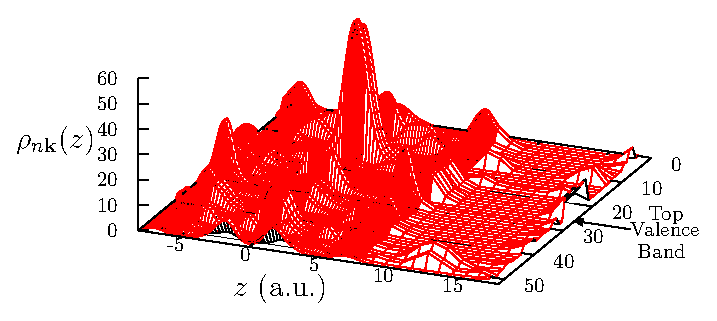
\includegraphics[scale=1.0]{plots/3drho}
\end{center}
\caption{$\rho_{n\bfk}(z)$ for the Si(111)As surface of the example 
  calcuated with spin-orbit interaction. 
}
\label{figrho}
\end{figure}

\item Integrated density  $\rho_{n\bfk}(z)=\int dx\int
  dy\,|\psi_{n\bfk}(\bfr)|^2$ (see Fig. \ref{figrho}) 

\begin{itemize}
\item
 write or generate \verb=case.klist_rho= with the
 $\bfk$-points where it
needs to be evaluated, typical the $\Gamma$ point and some other few
points of maximum
symmetry. \textcolor{red}{Modify}\verb=.machines_pmn= such that the
number of $\bfk$-points is the same as the number of CPU's.
\item run with option \verb=-m= and follow instructions.
\end{itemize}
\item After you are done with the calculation erase as follows:
\begin{itemize}
\item\verb=$PWD > =\textcolor{darkgreen}{run\_tiniba.sh -r} \textcolor{blue}{erase}

to erase the files in all the nodes.

\item\verb=$PWD > =\textcolor{darkgreen}{run\_tiniba.sh -r} \textcolor{blue}{erasescf}

to erase the SCF calculation.\textcolor{red}{WARNING: this erases the wave-function and may
 be better to keep it for future calculations, perhaps in a back-up HD}.

\end{itemize}

\end{enumerate}

\section{Benchmark Test}

Above example is run automatically by using and following the
instructions of\\
$\bullet$ \verb=$PWD >$TINIBA/utils/run-whole-enchilada-surface.sh=\\
where the output ought to be compared with benchmark results in order
to check that TINIBA${\reg}$ is working correctly.

However the calculation of $\chi^{\rmx\rmy\rmz}(2\go)$ for GaAs is a
better benchmark, since it is more sensitive to all the ingredients of
the calculation. It is run with\\
$\bullet$ \verb=$PWD >$TINIBA/utils/run-whole-enchilada-bulk.sh=\\

\section{Optics}
 
The program to run all the optical responses is\\
$\bullet$\verb=$TINIBA/utils/all_responses.sh=\\ 
which in turn runs\\
$\bullet$\verb=$TINIBA/utils/responses.sh=\\
To run it just execute\\
$\bullet$ \verb=$PWD > all_responses.sh= \\
and follow instructions. In particular one can calculate from all
valence bands to any number of conductions bands (\verb=-o 1=),
or from a given valence band to a given conduction band (\verb=-o 2=).

\begin{itemize}
\item For SHG bulk/surface use response 21/44. Both are coded in the
  Length Gauge. Response 42 only works
  for bulk and is coded the
  Velocity Gauge. Since it has to calculate extra commutators is
  slower than response 21. Thus use 42 only if you doubt your results
  and would like to get some reasurance that they are correctly
  calculated by 21.

\item The file for SHG has for columns\\\\
\begin{tabular}{|c|c|c|c|c|c|}\hline 
Column $\to$  & 1 & 2 & 3 & 4 & 5 \\\hline 
Quantity $\to$  & $\hbar\go$  & $\mathrm{Re}[\chi_{ijk}(1\go)]$ &
$\mathrm{Im}[\chi_{ijk}(1\go)]$ &
$\mathrm{Re}[\chi_{ijk}(2\go)]$ &
$\mathrm{Im}[\chi_{ijk}(2\go)]$\\\hline
\end{tabular} 
Units: pm/V\\
\textcolor{red}{So far it only works for one component of $\chi_{ijk}$.}

\item Degree of Spin Polarization (DSP), $\cald^a$.
\begin{enumerate}
\item \textcolor{red}{WARNING}: the factor of $(\hbar/2)$ is NOT
  included in $\zeta^{abc}$. However it is included in the expression
  for $\cald^a$, and thus the value of $\zeta^{abc}$ as it comes out
  of the code must be used to compute $\cald^a$. To report the value
  of $\zeta^{abc}$ one must multiply by $\hbar/2$ and use the
  appropriate S.I. units V$^{-2}$m$^{-1}$J.
\item For a surface calculation use a symmetric slab, i.e. same top
  and bottom surfaces.
\item Use \verb=dsp.sh= to gather the results for the DSP calculation. It
  does so for bulk (full) or layer-by-layer. The data is written as
follows:\\\\
\begin{tabular}{|c|c|c|c|c|c|}\hline
Column $\to$  & 1 & 2 & 3 & 4 &5 \\\hline
\verb=kk=$\to$  & $\hbar\go$  & $\xi_{xx}$  &
$\xi_{yy}$ &$\xi_{zz}$ & $\zeta_{ijk}$ \\ \hline
\end{tabular}\\
\item \verb=dsp.sh= uses the \verb=kk= response files and not the \verb=sm=
files. The onset of the DSP is very sharp and the \verb=sm= files
misscalculate it.
\item\verb=gnuplot> p 'dsp-file' u 1:(2*$5/($j+$k+eta)) w l=\\
where $j$ and $k$ are the corresponding columns (2,3 or 4) according to the $jk$
Cartesian components of $\zeta_{ijk}$. Also,
\verb=eta->0=, so {\it gnuplot} plots the DSP onset properly.
\item If you have calculated \verb=dsp.sh= with the \verb=full= option
  for a surface, i.e. the whole ``bulk-like''
 structure,
 then you must get the same result as with the
  \verb=half-slab= option, since both $\xi^{ab}$ and $\zeta^{abc}$ are
  twice as much for the whole slab than for the half-slab, but the
  factor of two cancels out when taking the ratio in the expression for $\cald^a$.
\end{enumerate}

\end{itemize}

\section{Examples}
\subsection{Bulk} 
For an example copy from \verb=$TINIBA/examples/surface/nospin/gaas=:\\
\verb=setUpAbinit_gaas.in= and \verb=gaas.xyz=. This is a
bulk GaAs crystal. See results in \verb=gaas/res= and Fig.~\ref{shg-bulk}.
\begin{figure}[t]
\begin{center}
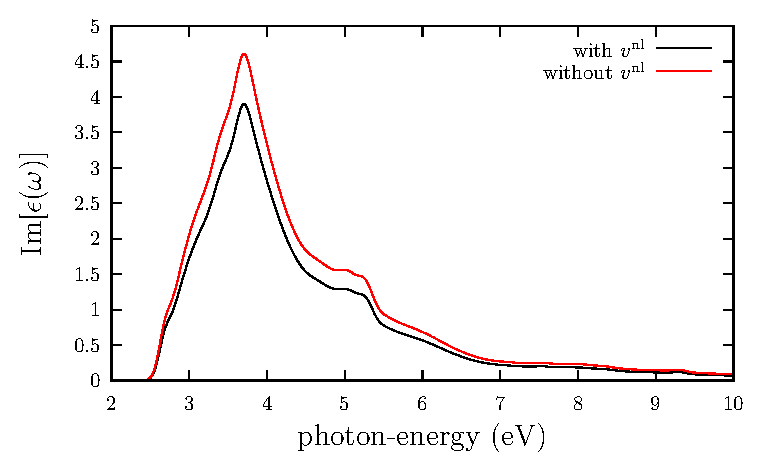
\includegraphics[scale=0.5]{plots/eps-bulk}
\end{center}
\caption{Im[$\ge(\go)$] for Si, $E_{cut}=10$ Ha and $N_k=29$.
With and without $\bfv^\nl_{nm}(\bfk)=(i/\hbar)\bra{n\bfk}[\hat V^\nl,\hat\bfr]\ket{m\bfk}$.
}
\label{si-bulk}
\end{figure}
\begin{figure}[t]
\begin{center}
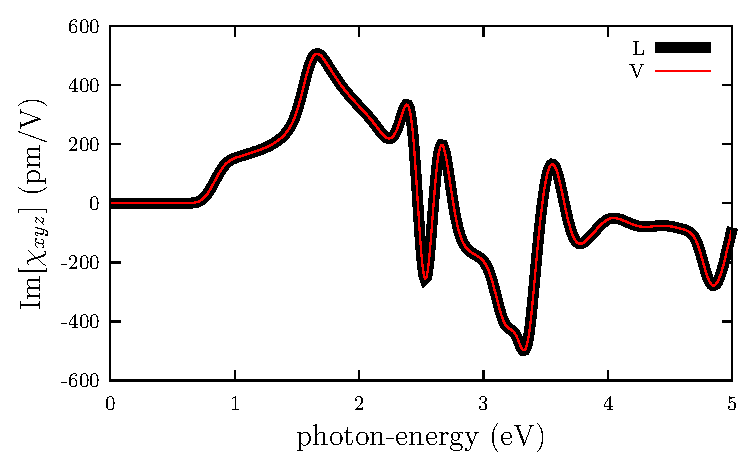
\includegraphics[scale=0.5]{plots/shg-bulk}
\end{center}
\caption{$\chi_{xyz}$ for GaAs, $E_{cut}=20$ Ha and $N_k=1661$. Both
  the length ($L$) and velocity ($V$) gauge results are shown.
The scissors shift is 1.051 eV.
}
\label{shg-bulk}
\end{figure}
\begin{figure}[t]
\begin{center}
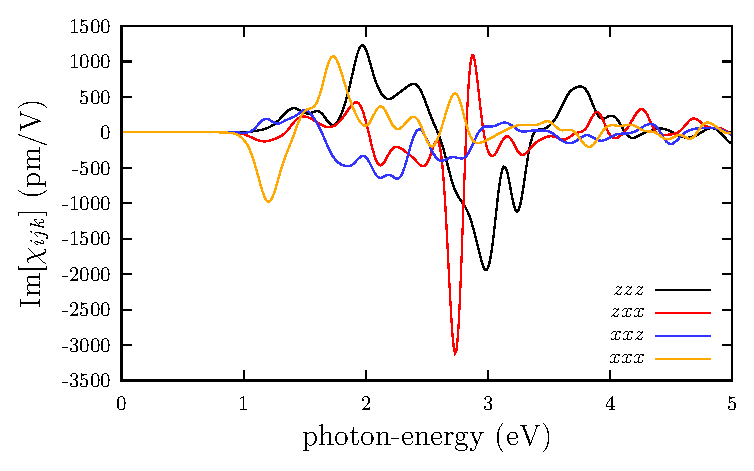
\includegraphics[scale=0.5]{plots/shg-surface}
\end{center}
\caption{Surface $\chi_{ijk}$ for all the allowed components of the
  si\_as\_6 example, $E_{cut}=5$ 
  Ha, $N_k=64$, and with a scissors shift of 0 eV. 
}
\label{shg-surface}
\end{figure}
\subsection{Surface}  
For an example copy from \verb=$TINIBA/examples/surface/nospin/si_as_6=:\\
\verb=setUpAbinit_si_as_6.in= and \verb=si_as_6.xyz=. This is a
Si(111)$1\times 1$:As surface with 4 layers of Si, one top and one bottom
layer of As. See results in \verb=si_as_6/res= and Fig.~\ref{shg-surface}.
\subsection{Surface Normalization}  
In Fig.~\ref{chil} we show Im[$\chi(\go)$] for the 
\verb=si_as_6=
 slab where three
different values of the supercell thickness, $L$, were chosen. As the
response is normalized with the volume $V=AL$ of the supercell, its value
decreases as $L$ is augmented. When, the results are multiplied by
$L$, as the area $A$ of the unit cell is fixed, we see that the
results  nicely converge. Then, the proper normalization is as follows
\begin{align}\label{m1}
\frac{L}{L_s}\left(\frac{1}{V}\right) 
=
\frac{L}{L_s}\left(\frac{1}{AL}\right) 
=\frac{1}{AL_s}\equiv\frac{1}{V_s}
,
\end{align}
where $L_s$ is the thickness of the material slab without the vacuum
layer, and then $V_s$ is the volume of the material slab. The 
\verb=all_response.sh= shell does the normalization automatically for
response \verb=24=.

\textcolor{red}{WARNING}: 
We mention that if one compares the response of the full slab with
that of the half-slab there is a factor of 2, once the full slab is
properly normalized as explained above. Then, 
$\chi_{\mathrm{full-slab}}(\omega)
=2 \chi_{\mathrm{half-slab}}(\omega)
$.

\textcolor{red}{WARNING}:
The code does NOT normalizes the full slab calculation, since  in a
slab calculation are ``layered'' responses what one ought to calculate. 
\begin{figure}[t]
\begin{center}
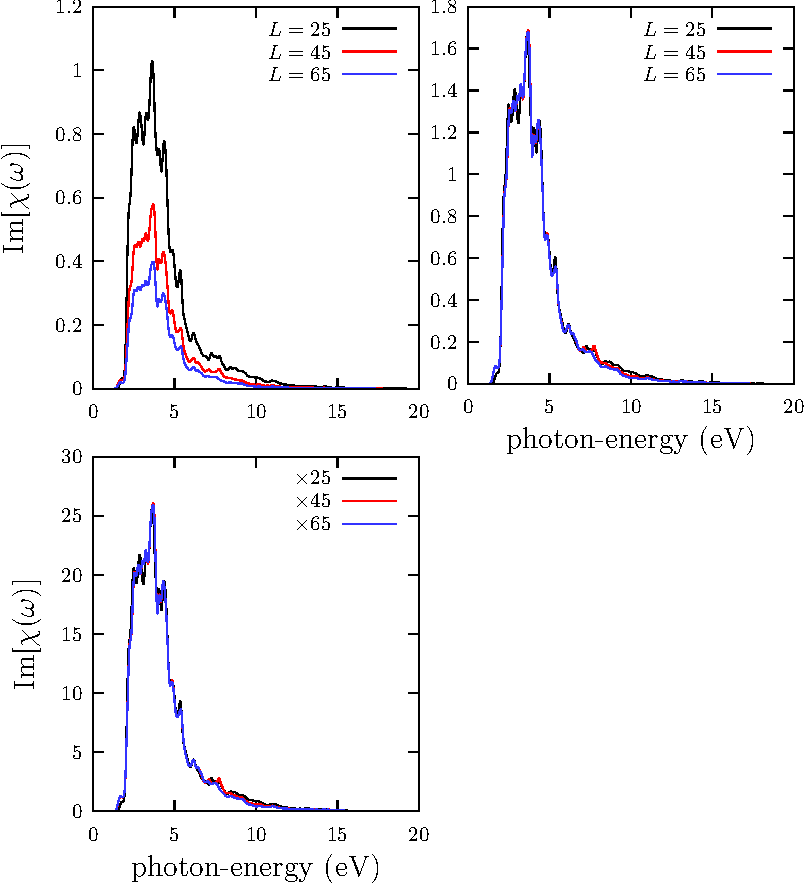
\includegraphics[scale=0.6]{plots/chi-layer}
\end{center}
\caption{Im[$\chi(\go)$] for three different supercells thickness
  $L$. Top-left panel without the normalization, bottom-left panel multiplied by
  $L$, and top-right panel scaled according to Eq.~\eqref{m1}. 
}
\label{chil}
\end{figure}


\section{For developers : how to include a new optics subroutine}
The optical response is calculated in two steps:\\
\begin{enumerate}
\item The calcualtion of integrand.
\item The integration over $k$.
\end{enumerate}
Both subrutines are implemented in Fortran code (thanks to Fred Nastos) and both 
are in \tiniba~package. In order to include the  subroutine for a new
response, we follow the following instructions. 
 
\subsection{Programs for Bulk and Layer-by-Layer response}
\label{sec:programs}

Do all the compilation in the \verb=master= node and in both 
\verb=SRC_1setinput=
and
\verb=SRC_2latam= directories.

There are two main steps in the calculation of the optical response:

\begin{enumerate}

\item The first one sets up the integrand. The
files are in\\
\verb=$TINIB/latm/SRC_1setinput=
\item The second one does the $\mathbf{k}$-integration. The files
  are in\\
\verb=$TINIBA/latm/SRC_2latam=
\end{enumerate}

Document the newest additions in between acronym marks like\\
\verb=#BMSd=\\
$\vdots$\\
\verb=#BMSu=\\
where \verb=d= is for down and \verb=u= is for up.

\begin{itemize}
%%%%%%%%%%
\item\verb=$TINIBA/latm/SRC_1setinput=
%%%%%%%%%%

\begin{enumerate}
\item In
  \verb=integrands.f90=\\
 include a CASE and the name of the subroutine, i.e \\
\verb=   CASE(21)=\\
\verb=   CALL SHG1L=\\
then write the subroutine itself. You can follow the structure from
  any other subroutine that works, like SHG1L. 

\item In \verb=inparams.f90= do the following
\begin{itemize}
\item In the \verb=MODULE inparams= 
add the response prefactor as a parameter, i.e.\\
\verb=REAL(DP),PARAMETER::shg1_factor= $=\cdots$\\
This is a numerical factor such that the response gives the
appropriate S.I. units, see Sec.~\ref{units}.  

\item In the \verb=MODULE inparams=  add the response prefactor in the array\\
\verb=spectrum_factor(number_of_known_spectrum_types)==\\       
$\vdots$\\
\verb=!    21           22          23           =\\
\verb=  shg1_factor, shg2_factor, leo_factor=,$\cdots$\\
$\vdots$\\
where it is {\bf very important} that the number chosen for the
\verb=CASE= of the response, i.e. 21, coincides with the position-entree in
the array.
\item In the \verb=SUBROUTINE readSpectrumFile= add the \verb=CASE=
 number in the appropriate response, where \verb=dims= is the rank
 and \verb=length= is the total number of
 Cartesian components of
the tensor's response, i.e.\\
$\vdots$
\begin{verbatim}
 CASE(21,42,44)
  WRITE(6,*) "Second-harmonic generation"
  dims = 3
  length = 27
\end{verbatim}
$\vdots$

since the rank is 3 and 3$^3$=27

\item In the \verb=SUBROUTINE deltaFactor= add the 
correct\\ \verb=deltaFunctionFactor==1 or 2\\ for 1-$\omega$ and 
2-$\omega$ transitions, respectively.
 The default value is\\
\verb=deltaFunctionFactor==1 for 1-$\omega$ response terms.
Otherwise include the response \verb=CASE= number, i.e.,\\
$\vdots$
\begin{verbatim}
 CASE(22,43,45)!shg 2-omega terms
   deltaFunctionFactor=2
 END SELECT
\end{verbatim}
$\vdots$

since \verb=shg2= is a 2-$\omega$ response term.
\end{itemize} 

\item In \verb=set_input_bin.f90=
 the ``\verb=all='' the ``\verb=standard='' and the \\ 
``\verb=layer-by-layer=''
position and momentum matrix elements are set into arrays so they can be used by the 
\verb=intergands.f90= file. 

Most of the responses already have the required
matrix elements so this file should not be changed unless new matrix
elements are needed.

The newest additions are documented between\\
\verb=#BMSd=\\
$\vdots$\\
\verb=#BMSu=\\
marks, so one can check how new matrix elements can be included.
%Check that the momentum-matrix elements are
%properly renormalized due to the scissors shift. 

\item In \verb=symmetry_operations.f90= include the \verb=CASE= number
  of the response in the appropriate transformation (linear,
  secon-order, etc.), i.e.\\
$\vdots$
\begin{verbatim}
  CASE(21,22,42,43,44,45)
   CALL transformationSecondOrderResponse(i_spectra)
\end{verbatim} 
$\vdots$

The symmetries are obtained from the file generated by the LDA program
and they obtain the following array
\begin{equation}\label{uno}
R_{ij\cdots}=\sum_{\mathrm{ab}\cdots}M_{i\mathrm{a}} M_{j\mathrm{b}}\cdots
,
\end{equation}
where the {\it italic} Cartesian subindices of $R_{ij\cdots}$ are chosen by the
tensor component to be calculated, \verb=-t= option, 
and the $\mathrm{roman}$
Cartesian subindices of the rotation matrices $M_{i\mathrm{a}}$ are
summed over.

The following four files basically do not need to be changed.
\item In \verb=arrays.f90= the arrays are allocated and de-allocated
  for things like the momentum matrix elements. So far it has all the
  arrays needed for many responses, so most likely there is no need to
  edit this file. The file also reads the LDA energies and scissored
  energies with the value of the provided scissor correction.

The newest additions are documented between\\
\verb=#BMSd=\\
$\vdots$\\
\verb=#BMSu=\\
marks.
%Perhaps the layered spin injection response needs to add the
%appropriate array for the layered spin matrix elements.

\item \verb=constants.f90= has only constants and there is no need to
modify it.
\item \verb=file_control.f90= controls the flow of the calculation,
there is no need to
modify it.
\item \verb=functions.f90= calculates the standard and  layer-by-layer position
  matrix elements, the generalized derivatives of the position matrix
  elements, and other goodies not required. 
There is no apparent need to
modify it unless one wants to change the layer-by-layer response.
The newest additions are documented between\\
\verb=#BMSd=\\
$\vdots$\\
\verb=#BMSu=\\
marks.

\item \verb=$TINIBA/clustering/itaxeo/set.pl= This \verb=perl= script puts together the
  \verb=setUpAbinit_case.in= files to be run. If changes are needed follow the
newest additions documented between\\
\verb=#BMSd=\\
$\vdots$\\
\verb=#BMSu=\\
marks.

\item Compilation
\begin{itemize}
\item run \verb=compiler_all.sh= to compile in the three plataforms
\item the executable is one directory down, i.e.\\
\verb=../set_input_all=
\item you may want to change the compiler and compilation flags in:\\
\verb=MakefileAll=
\end{itemize}

\end{enumerate}

%%%%%%%%%%
\item\verb=$TINIBA/latm/SRC_2latam=
%%%%%%%%%%
\begin{enumerate}
\item\verb=inparams.f90= is the same as that of\\
\verb=$TINIBA/latm/SRC_1setinput=\\
it is linked so if you change it in \verb=SRC_1setinput=
 you must compile in \verb=SRC_2latam=!
\item \verb=tetra_method.f90=
\begin{itemize}
\item does the integration using the Tetrahedral Method.
\item you may want to play with the 
\verb=SUBROUTINE Which_Transitions= to chose particular transitions,
i.e. look in \verb=tetra_method_vc.f90=, but be sure that is
implemented for 2-$\omega$ terms.
\end{itemize}

\item \verb=constants.f90= has only constants and there is no need to
modify it.
\item \verb=globals.f90= global statements and there is no need to
modify it.
\item \verb=piksort.f90= there is no need to
modify it.
\item Compilation
\begin{itemize}
\item run \verb=compiler_all.sh= to compile in the three plataforms
\item the executable is one directory down, i.e.\\
\verb=../tetra_method_all=
\item you may want to change the compiler and compilation flags in:\\
\verb=MakefileAll=
\end{itemize}

\end{enumerate}

\item Name for the Response

\begin{itemize}
\item To include a new response once is coded as explained in
 Sec. \ref{sec:programs}, 
the name of the response (i.e. \verb=rhomm=) 
 must go in the following files complying with the particular context 
\begin{itemize}
\item 
\verb=$TINIBA/utils/responses.txt=  
and add the
 number and name of the respnse, perhaps you may want to modify\\
\verb=$TINIBA/utils/print_responses.pl=\\ for fine tunning
of the displayed text. 
\item\textcolor{red}{NOTE:}The names that appear in
  \verb=responses.txt= are the ones used, \verb=verbatim=, for the name
  of the calculated responses. Thus for a different name for the same
  response just modify this file!
\end{itemize}
\item In \verb=$TINIBA/utils/responses.sh=
\begin{enumerate}
\item add the response number around the lines\\
\Verb+if [ $lt = 'total' ]+ and \Verb+if [ $lt = 'layer' ]+
\\
if the response is a layer response. 
\item around the line \\
\Verb+for ij in ${scases[@]}+
\\
add the response number if no Kramers-Kronig (KK) transformation is
needed. 

\item \textcolor{blue}{HELP:} look for 
\verb=#BMSd 09/sep/2016= that account for the latest modification to
include the spin current injection $\mu^{abcd}$ bulk and layer response.

\end{enumerate}
\end{itemize}

%%%
\end{itemize}


\subsection{Shell for Bulk and Layer-by-Layer response}

\begin{itemize}

\item To run the optical responses execute and follow the instruction of the bash \verb=shell=:

  \verb=$TINIBA/utils/all_responses.sh=\\
which uses\\
\verb=$TINIBA/utils/responses.sh=

\item To include a new response once is coded as explained in
 Sec. \ref{sec:programs} 

\begin{itemize}
\item edit
\verb=$TINIBA/utils/responses.txt=  
and add the
 number and name of the respnse, perhaps you may want to modify\\
\verb=$TINIBA/utils/print_responses.pl=\\ for fine tunning
of the displayed text.
\end{itemize}
\item The SHG is calculated with \verb=CASE==21 and does both 1-$\go$
  and 2-$\go$ terms.
\end{itemize}

\subsection{Formulas}


These are the coded formulas: ($\go_{nm}^{Sigma}$ are the scissors energies) 

\begin{enumerate}

\item Linear response (See Sipe and Shkrebtii PRB {\bf 61}, 5337 (2000) Eq. 34
% \begin{equation*}\label{chi}
% \mathrm{Im}[\chi^{ij}(\go)]=\frac{e^2\pi}{\hbar}
% \int \frac{d\bfk}{8\pi^3}
% \sum_{nm} 
% f_{nm} 
% r^i_{nm}(\bfk)r^j_{mn}(\bfk)\gd(\go_{mn}(\bfk)-\go)
% ,
% \end{equation*}  
%where $m=c$ and $n=v$ for the resonant condition with $\go>0$),
\begin{equation}\label{chif}
\mathrm{Im}[\chi^{\rma\rmb}(-\go;\go)]
=\frac{\pi e^2}{\hbar}
\int \frac{d\bfk}{8\pi^3}
\sum_{vc} 
r^{\rma}_{vc}(\bfk)r^{\rmb}_{cv}(\bfk)\gd(\go^\gs_{cv}(\bfk)-\go)  
.  
\end{equation}  

Static response:
\begin{equation*}\label{chif0}
\chi^{\rma\rmb}(0;0)=\frac{e^2}{\hbar}
\int \frac{d\bfk}{8\pi^3}
\sum_{vc}\frac{2}{\go^\gs_{cv}}
\mathrm{Re}[r^{\rma}_{vc}(\bfk)r^{\rmb}_{cv}(\bfk)]
. 
\end{equation*} 
The prefactor (PF) of $\chi^{\rma\rmb}(0;0)$ is
\begin{align}\label{mcv1}
\mathrm{PF}[\chi^{\rma\rmb}(0;0)]=\frac{1}{\pi}
\mathrm{PF[Im}(\chi^{\rma\rmb}(-\go;\go))]
.
\end{align}
For the layer response we replace $r^{\rma}_{vc}(\bfk)\to{\cal 
 R}^{(\ell)\rma}_{vc}(\bfk)$ see Mendoza et al, Phys. Rev. B {\bf 74},
075318 (2006). 

\item Carrier injection rate: is defined through,
\begin{align}\label{cir}
\dot n(\go)=\xi^{ij}(\go)E^i(-\go)E^j(\go)  
,
\end{align} 
where is better to redefine it as 
\begin{align}\label{cir}
\dot{\tilde n}=
\frac{\hbar}{2}\dot 
n=\tilde\xi^{ab}E^a(-\go)E^b(\go)
,
\end{align}
i.e. in $\hbar/2$ units, where
$\tilde\xi^{ab}=(\hbar/2)
\xi^{ab}$, and
\begin{equation}\label{chifp}
\tilde\xi^{\rma\rmb}(\go)=\frac{\pi e^2}{\hbar}
\int \frac{d\bfk}{8\pi^3}
\sum_{vc}
r^{\rma}_{vc}(\bfk)r^{\rmb}_{cv}(\bfk)\gd(\go_{cv}(\bfk)-\go)
.
\end{equation} 
For the layer response:
\begin{equation*}\label{xizn}
\tilde\xi^{ab}(\ell;\go)
=
\frac{\pi e^2}{\hbar}
\int\frac{d^3k}{8\pi^3}
\sum_{vcc'}
\frac{1}{2}\mathrm{Re}\Big[
\rho_{cc'}(\ell)    
r^a_{vc} 
r^b_{c'v}
+
\rho_{c'c}(\ell) 
r^a_{vc'} 
r^b_{cv}
\Big]
\gd(\omega-\omega_{cv})
.
\end{equation*}
We notice that $\tilde\xi^{ab}(\go)=\mathrm{Im}[\chi^{ab}(\go)]$, with
$\ge^{ab}(\go)=1+4\pi\chi^{ab}(\go)$, however 
$\tilde\xi^{ab}(\ell;\go)\neq\mathrm{Im}[\chi^{ab}(\ell;\go)]$!!!
Therefore, for a \textcolor{red}{bulk} calculation, one must calculate
$\mathrm{Im}[\chi^{ab}(\go)]$ for $\dot n(\go)$.
Also,
\begin{align}\label{nn.11}
\mathrm{Im}[\ge^{\rma\rmb}(\go)]
&=
4\pi\mathrm{Im}[\chi^{\rma\rmb}(\go)]
=
2\pi\hbar\xi^{\rma\rmb}(\go)
\nonumber\\
\Rightarrow 
\xi^{\rma\rmb}(\go) 
&=
\frac{2}{\hbar}\mathrm{Im}[\chi^{\rma\rmb}(\go)],
\nonumber\\
\Rightarrow 
\tilde\xi^{\rma\rmb}(\go) 
&=
\mathrm{Im}[\chi^{\rma\rmb}(\go)],
\end{align}


\item Second Harmonic Generation
\begin{itemize}
\item Velocity-Gauge 

The SHG $\chi_{\rmv}^{\rma\rmb\rmc}(2\go)$ is programmed within the velocity-gauge
 according to Phys.  Rev. B {\bf 80}, 155205-1-13 (2009).
\begin{eqnarray*}
&&\mbox{Im}\lbrack \chi _{\mathrm{v}}^{abc}(-2\omega;\omega,\omega)] 
=\frac{\pi
|e|^{3}}{2\hbar ^{2}}\int \frac{d^{3}k}{8\pi ^{3}}\Big[\sum_{vc}\frac{16}{(
\omega_{cv}^{S})^{3}}\Big(\sum_{c^{\prime }}\frac{\mbox{Im}\lbrack
v_{vc}^{\Sigma ,a}\{v_{cc^{\prime }}^{\Sigma ,b}v_{c^{\prime }v}^{\Sigma
,c}\}]}{\omega_{cv}^{S}-2\omega_{c^{\prime }v}^{S}}  \notag  \label{imchicf} \\
&-&\sum_{v^{\prime }}\frac{\mbox{Im}\lbrack v_{vc}^{\Sigma
,a}\{v_{cv^{\prime }}^{\Sigma ,b}v_{v^{\prime }v}^{\Sigma ,c}\}]}{\omega
_{cv}^{S}-2\omega_{cv^{\prime }}^{S}}\Big)\delta(\omega_{cv}^{S}-2\omega)  \notag \\
&+&\sum_{(vc)\neq\ell }\frac{1}{(\omega_{cv}^{S})^{3}}\Big(\frac{\mbox{Im}\lbrack
v_{\ell c}^{\Sigma ,a}\{v_{cv}^{\Sigma ,b}v_{v\ell }^{\Sigma ,c}\}]}{\omega
_{c\ell }^{S}-2\omega_{cv}^{S}}-\frac{\mbox{Im}\lbrack v_{v\ell }^{\Sigma
,a}\{v_{\ell c}^{\Sigma ,b}v_{cv}^{\Sigma ,c}\}]}{\omega_{\ell v}^{S}-2\omega
_{cv}^{S}}\Big)\delta(\omega_{cv}^{S}-\omega)  \notag \\
&-&\sum_{vc}\frac{1}{(\omega_{cv}^{S})^{3}}\Big(4\mbox{Re}\lbrack \
v_{vc}^{\Sigma ,a}\{\mathcal{F}_{cv}^{bc}\}]\delta(\omega_{cv}^{S}-2\omega)+\mbox{Re}
\lbrack \{\mathcal{F}_{vc}^{ab}v_{cv}^{\Sigma ,c}\}]\delta(\omega_{cv}^{S}-\omega)
\Big)\Big].
\end{eqnarray*}
Programs: \verb=shg1v= and \verb=shg2v=

\item Length-Gauge: 
Layered response by bms-unpublished. See\\
 \verb=/Users/bms/research/austin/shg/shg-notes/shg-layer-nonlocal.pdf=
\begin{equation}\label{calvimchiewn}
\mathrm{Im}[\chi_{e,\rma\rmb\rmc,\go}^{s,\ell}] =
\frac{\pi |e|^3}{2\hbar^2}\sum_{vc\bfk}\sum_{l\neq(v,c)}\frac{1}{\omega^\gs_{cv}}
\left[
\frac{\mathrm{Im}[\mathcal{V}^{\gs,\text{a},\ell}_{lc}\{r^{\rmb}_{cv}r^{\rmc}_{vl}\}]}
{(2\go^\gs_{cv}-\go^\gs_{cl})} 
-\frac{\mathrm{Im}[\mathcal{V}^{\gs,\text{a},\ell}_{vl}\{r^{\rmc}_{lc}r^{\rmb}_{cv}\}]}
{(2\go^\gs_{cv}-\go^\gs_{lv})}
\right]\gd(\go^\gs_{cv}-\go),
\end{equation}  
\begin{equation}\label{calvimchiwn}
\mathrm{Im}[\chi_{i,\text{a}\text{b}\text{c},\omega}^{s,\ell}]
= \frac{\pi\vert e\vert^3}{2\hbar^2}\sum_{cv\mathbf{k}}\frac{1}{(\omega^\gs_{cv})^{2}}
\left[
\mathrm{Re}\left[\left\{r^{\text{b}}_{cv}\left(\mathcal{V}^{\gs,\text{a},\ell}_{vc}\right)_{;k^{\text{c}}}\right\}\right]
+\frac{\mathrm{Re}\left[\mathcal{V}^{\gs,\text{a},\ell}_{vc}\left\{r^{\text{b}}_{cv}
\Delta^{\text{c}}_{cv}\right\}\right]}{\omega^\gs_{cv}} 
\right]\delta(\omega^\gs_{cv}-\omega),
\end{equation}
\begin{equation}\label{calvimchie2wn}
\mathrm{Im}[\chi_{e,\rma\rmb\rmc,2\go}^{s,\ell}] =
-\frac{\pi |e|^3}{2\hbar^2}\sum_{vc\bfk}\frac{4}{\omega^\gs_{cv}}
\left[
\sum_{v'\ne
  v}\frac{\mathrm{Im}[\mathcal{V}^{\gs,\text{a},\ell}_{vc}\{r^{\rmb}_{cv'}r^{\rmc}_{v'v}\}]}
{2\go^\gs_{cv'}-\go^\gs_{cv}}
- \sum_{c'\ne
  c}\frac{\mathrm{Im}[\mathcal{V}^{\gs,\text{a},\ell}_{vc}\{r^{\rmc}_{cc'}r^{\rmb}_{c'v}\}]}
{2\go^\gs_{c'v}-\go^\gs_{cv}}
\right]\gd(\go^\gs_{cv}-2\go),
\end{equation}
and
\begin{equation}\label{calvimchi2wn}
\mathrm{Im}[\chi_{i,\text{a}\text{b}\text{c},2\omega}^{s,\ell}] 
=
 \frac{\pi \vert
   e\vert^{3}}{2\hbar^2}\sum_{vc\mathbf{k}}\frac{4}{(\omega^\gs_{cv})^{2}}
\left[\mathrm{Re}\left[\mathcal{V}^{\gs,\text{a},\ell}_{vc}\left\{\left(r^{\text{b}}_{cv}\right)_{;k^{\text{c}}}
\right\}\right] -
\frac{2\mathrm{Re}\left[\mathcal{V}^{\gs,\text{a},\ell}_{vc}\left\{r^{\text{b}}_{cv}
\Delta^{\text{c}}_{cv}\right\}\right]}{\omega^\gs_{cv}}\right]\delta(\omega^\gs_{cv}-2\omega)
,
\end{equation}


\end{itemize}
Programs: \verb=shg1l= and \verb=shg2l= for bulk, i.e. ${\cal
  R}^{\rma(\ell)}_{vc}\to r^\rma_{vc}$.\\
\verb=shg1c= and \verb=shg2c= for layered.


\item Injection current  

\begin{equation}\label{etaell}
\eta^{\rma\rmb\rmc}(\ell|0;\go,-\go)  
=
\frac{i\pi e^3}{\hbar^2}
\intk  
\sum_{vc}
\gD_{cv}^{\rma,\ell}(\bfk)  
\mathrm{Im}
\big[  
r^{\rmb}_{cv}(\bfk)  
r^{\rmc}_{vc}(\bfk)  
\big]
\gd(\go_{cv}(\bfk)-\go)  
.  
\end{equation}  
For the bulk response we replace 
$\gD_{cv}^{\rma,\ell}(\bfk) \to \gD_{cv}^{\rma}(\bfk)$, with
\begin{align}\label{ic.1}
\gD_{cv}^{\rma,\ell}(\bfk) 
=\calv_{cc}^{\rma,\ell}(\bfk) -\calv_{vv}^{\rma,\ell}(\bfk) 
.
\end{align}

\textcolor{red}{??NOTE??}: run the code as it is, then with the new
$\gD_{cv}^{\rma,\ell}(\bfk)$, to see the 
changes, and thus discontinue the use of option \verb=-l= and \verb=curMatElem=
$\cdots$ since $\calc^\ell_{nm}$ needs to be used for the correct
calculation of
$\gD_{cv}^{\rma,\ell}(\bfk)$.

\item Shift current

\begin{equation}\label{sigma}
\sigma^{\rma\rmb\rmc}_2(\ell|0;\go,-\go) 
=
\frac{\pi e^3}{\hbar^2}
\intk 
\sum_{vc}
\mathrm{Im}
\big[ 
r^{\rmb}_{cv}(\bfk) 
r^{\rmc}_{vc;\rma}(\bfk) 
-
r^{\rmc}_{vc}(\bfk) 
r^{\rmb}_{cv;\rma}(\bfk) 
\big]
\gd(\go_{cv}(\bfk)-\go) 
. 
\end{equation} 


\item Spin injection

\begin{align}\label{zetaabci}
\zeta^{\mathrm{abc}}(\omega)
&=
\frac{i\pi e^2}{\hbar^2}
\int\frac{d^3k}{8\pi^3}
\sum_{vcc'}\,'\,
\mathrm{Im}\Big[S^{\mathrm{a}}_{c'c}(\mathbf{k}) r^{\mathrm{b}}_{vc'}(\mathbf{k}) r^{\mathrm{c}}_{cv}(\mathbf{k}) 
\nonumber\\
&+ 
S^{\mathrm{a}}_{cc'}(\mathbf{k}) r^{\mathrm{b}}_{vc}(\mathbf{k}) r^{\mathrm{c}}_{c'v}(\mathbf{k})\Big]
\delta(\omega_{cv}(\mathbf{k})-\omega) 
\nonumber\\
&=
\frac{i\pi e^2}{2\hbar}
\int\frac{d^3k}{8\pi^3}
\sum_{vcc'}\,'\,
\mathrm{Im}\Big[\gs^{\mathrm{a}}_{c'c}(\mathbf{k})
  r^{\mathrm{b}}_{vc'}(\mathbf{k}) r^{\mathrm{c}}_{cv}(\mathbf{k})  
\nonumber\\
&+ 
\gs^{\mathrm{a}}_{cc'}(\mathbf{k}) r^{\mathrm{b}}_{vc}(\mathbf{k})
  r^{\mathrm{c}}_{c'v}(\mathbf{k})\Big] 
\delta(\omega_{cv}(\mathbf{k})-\omega) 
\end{align}
Notice that the units of $\zeta^{\rma\rmb\rmc}(\go)$ have a $\hbar/2$
factor coming from the spin matrix elements $S^{\rma}_{cc'}$ (recall
that
$\hat \bfS=(\hbar/2)\hat\bfgs$), besides the other units.
The degree of spin polarization is defined as
\begin{equation}\label{dps}
{\cal
  D}=\frac{2\zeta^{\rmz\rmx\rmy}}{\hbar(\xi^{\rmx\rmx}+\xi^{\rmy\rmy})/2}
=\frac{2\zeta^{\rmz\rmx\rmy}}{(\tilde\xi^{\rmx\rmx}+\tilde\xi^{\rmy\rmy})}
,\nonumber
\end{equation}    
and it is a dimensionless quantity, as it must. 

For the layered response we replace 
$S^{\rma}_{cc'}(\bfk)\to {\cal  S}^{\ell,\rma}_{cc'}(\bfk)$.  


\item Spin Current Density

\begin{align}\label{ee.00}
\mu^{\mathrm{abcd}}=
\frac{\pi e^2}{\hbar^2}\int \frac{d^3k}{8\pi^3}
\sum'_{vcc'}\mathrm{Re}
[
\bra{c'\bfk}\hat v^{\gS,\rma}\hat S^\rmb\ket{c\bfk}
\,r^\rmc_{vc'}(\bfk) r^\rmd_{cv}(\bfk)  
+ (\rmc\leftrightarrow\rmd)  
]\gd(\go_{cv}(\bfk)-\go),
\end{align} 
where
\begin{align}\label{ee.1}
\bra{c'\bfk}\hat v^{\gS,\rma}\hat S^\rmb\ket{c\bfk}
&
=\frac{\hbar}{2}
\sum_n \bra{c'\bfk}\hat v^{\gS,\rma}\ket{n\bfk}\bra{n\bfk}\hat \gs^\rmb\ket{c\bfk}
\nonumber\\
&
=\frac{\hbar}{2}
\sum_n v^{\gS,\rma}_{c'n}(\bfk)\gs^\rmb_{nc}(\bfk)
,
\end{align}
then,
\begin{align}\label{ee.0}
\mu^{\mathrm{abcd}}=
\frac{\pi e^2}{2\hbar}\int \frac{d^3k}{8\pi^3}
&\sum'_{cc'}\mathrm{Re}\Big[
\sum_n 
v^{\gS,\rma}_{c'n}(\bfk)\gs^\rmb_{nc}(\bfk)
\nonumber\\
&\times\sum_v\Big(
r^\rmc_{vc'}(\bfk) r^\rmd_{cv}(\bfk) 
+ \,r^\rmd_{vc'}(\bfk) r^\rmc_{cv}(\bfk) 
\Big) 
\Big]\gd(\go_{cv}(\bfk)-\go),
\end{align}
where $n$ cover all valence and conduction states. We leave the
$\hbar/2$ out of the units of $\mu^{\mathrm{abcd}}$.

\end{enumerate}

\subsection{Units}\label{units}
 
\begin{enumerate}

\item {\bf S.I. and Gaussian units}


In general, there are two possibilities to define the
  polarization,
\begin{align}\label{u.69}
\tilde P&=\varepsilon_0\Big(\chi^{(1)}\tilde E+\chi^{(2)}\tilde E^2+\cdots\Big) 
\\
&\text{or}
\nonumber\\\label{u.69n}
\tilde P&=\tilde\chi^{(1)}\tilde E+\tilde\chi^{(2)}\tilde E^2+\cdots  
,
\end{align}  
where $\varepsilon_0=8.85 \times 10^{−12}$ F/m, is the permitivity of free space.
The units of $\tilde P$ 
are those of charge times distance over
volume, then 
\begin{align}\label{u.691}
[\tilde P]&=[\varepsilon_0]\Big([\chi^{(1)}][\tilde E]+[\chi^{(2)}][\tilde E^2]+\cdots\Big) 
\nonumber\\
\frac{\text{C}}{\text{m}^2}&=
\frac{\text{F}}{\text{m}}
\Big([\chi^{(1)}]\frac{\text{V}}{\text{m}}
+[\chi^{(2)}]\frac{\text{V}^2}{\text{m}^2}
+\cdots\Big) 
\nonumber\\
\frac{\text{C}}{\text{m}^2}&=
\frac{\text{C}}{\text{m}^2}
[\chi^{(1)}]
+[\chi^{(2)}]\frac{\text{CV}}{\text{m}^3}
+\cdots 
\nonumber\\
&\text{or}
\nonumber\\
[\tilde P]&=[\tilde\chi^{(1)}][\tilde E]+[\tilde\chi^{(2)}][\tilde E^2]+\cdots 
\nonumber\\
\frac{\text{C}}{\text{m}^2}&=
[\tilde\chi^{(1)}]\frac{\text{V}}{\text{m}}
+[\tilde\chi^{(2)}]\frac{\text{V}^2}{\text{m}^2}
+\cdots 
,
\end{align}  
since $[\tilde E]=$V/m and F=C/V. We obtain that,
\begin{align}\label{u.692}
[\chi^{(1)}]=\text{dimensionless}
&\quad 
[\chi^{(2)}]=\frac{\text{m}}{\text{V}}
\nonumber\\
[\tilde\chi^{(1)}]=\frac{\text{C}}{\text{mV}}=\frac{\text{F}}{\text{m}}
&\quad 
[\tilde\chi^{(2)}]=\frac{\text{C}}{\text{V}^2}
,
\end{align}
and the higher order $\chi$'s could be worked out along the same
line. Above units are in the MKS system. In the cgs system, 
$\tilde E$, $\tilde P$, $\tilde D$, $\tilde B$, $\tilde H$, and
$\tilde M$, have the same units; in particular, the units of $\tilde
E$ and $\tilde P$ are given by,
\begin{align}\label{u.2}
[\tilde E]=[\tilde P]=
\frac{\text{statvolt}}{\text{cm}}
=
\frac{\text{statcoulomb}}{\text{cm}^2}
=
\left(\frac{\text{erg}}{\text{cm}^3}\right)^{1/2}
,
\end{align} 
and therefore 
\begin{align}\label{u.3}
[\tilde \chi^{(1)}]&=\text{dimensionless}
\nonumber\\
[\tilde \chi^{(2)}]&=
\frac{\text{cm}}{\text{statvolt}}
=\left(\frac{\text{erg}}{\text{cm}^3}\right)^{-1/2}
,
\end{align}
where the units are referred simply as electrostatic units (esu). 

Con convert from the esu system to the MKS system, we write
\begin{align}\label{u.5}
\tilde P&=\varepsilon_0
\chi^{(1)}\tilde E\Big(1+\frac{\chi^{(2)}}{\chi^{(1)}}\tilde E+\cdots\Big) \quad(\text{MKS})
\nonumber\\
\tilde P&=\tilde\chi^{(1)}\tilde E\Big(1+\frac{\tilde\chi^{(2)}}{\tilde\chi^{(1)}}\tilde E+\cdots  \Big)\quad\text{(gaussian)}
,
\end{align} 
where the power series must be identical in each of these equations.
Using the fact that 1 statvolt=300 V, and Eq.~\eqref{u.2} we find that 
\begin{align}\label{u.10}
\tilde E\, (\text{MKS})=3\times 10^4\tilde E \,(\text{gaussian})
.
\end{align}
To relate the MKS with the gaussian susceptibilities, we proceed as
follows,
\begin{align}\label{u.11}
\tilde D &= \tilde E + 4\pi\tilde P 
=\tilde E\big(1+4\pi\tilde \chi^{(1)})\quad\text{gaussian}
\nonumber\\
\tilde D &= \varepsilon_0\tilde E + \tilde P 
=\varepsilon_0\tilde E\big(1+ \chi^{(1)})\quad\text{MKS}
,
\end{align}   
from where
\begin{align}\label{u.12}
\chi^{(1)}\,(\text{MKS})= 
4\pi\tilde \chi^{(1)}\,(\text{gaussian})  
.  
\end{align}   
Using Eq.~\eqref{u.10} and Eq.~\eqref{u.5}, we find that
\begin{align}\label{u.13}
\chi^{(2)}\,(\text{MKS})=
\frac{4\pi}{4\times 10^4}\tilde \chi^{(2)}\,(\text{gaussian}) 
, 
\end{align}  
which can be generalized to
\begin{equation}\label{si0}
\chi_{\mathrm{S.I.}}^{(j)}=\frac{4\pi}{(3\times 
 10^4)^{j-1}}\tilde\chi^{(j)}_{\mathrm{cgs}}
,
\end{equation} 
with $j$ the order of the response.  Now, from Eqs.~\eqref{u.69}-\eqref{u.69n}, in
the MKS system
\begin{align}\label{u.20}
\tilde\chi^{(j)}_{\text{S.I.}}=\varepsilon_0\chi^{(j)}_{\text{S.I.}}
,
\end{align}
and the equivalent of Eq.~\eqref{si0} is
\begin{equation}\label{si.2}
\tilde\chi_{\mathrm{S.I.}}^{(j)}=\frac{4\pi\ge_0}{(3\times 
 10^4)^{j-1}}\tilde\chi^{(j)}_{\mathrm{cgs}} \times 
\frac{\text{m}^{j-2}\text{C}}{\text{V}^j}
,
\end{equation}  
where the 
$\text{m}^{j-2}\text{C}/\text{V}^j$
units already have those of $\varepsilon_0$, and thus we use
the following numerical factor for
\begin{equation*}\label{is}
\frac{1}{4\pi\ge_0}=9\times 10^9%\frac{Nm^2}{C^2}
,
\end{equation*} 
with which
\begin{equation}\label{si}
\tilde\chi_{\mathrm{S.I.}}^{(j)}=
\frac{1}{9\times 10^9}\frac{1}{(3\times 
 10^4)^{j-1}}\tilde\chi^{(j)}_{\mathrm{cgs}} \times 
\frac{\text{m}^{j-2}\text{C}}{\text{V}^j}
,
\end{equation} 
is the conversion factor (including the S.I. units) in going from cgs
to S.I., where we follow the representation of
Eq.~\eqref{u.69n} for the polarization; then,
\begin{align}\label{u.691}
[\tilde\chi^{(j)}_{\mathrm{S.I.}}]
&=
\frac{\text{m}^{j-2}\text{C}}{\text{V}^j}
,
\end{align}

Then, we every response, $\calr$, calculated by \tiniba, has a
prefactor $\gamma$ and the units in the S.I. system of units, given in
the following items. $\gamma$ is coded in
\verb=$TINIBA/latm/SRC_1setinput/inparams.f90=. 

\item {\bf Response's prefactors}\\

Any response $\calr$ calculated by \tiniba, is written as
\begin{align}\label{pf.1}
\calr=\gamma\,\tilde\calr
,
\end{align}
where $\tilde\calr$ is the quantum mechanical expression obtained for
$\calr$, and $\gamma$ is the prefactor that one obtains, by using the
Gaussian units of the matrix elements that enter into $\tilde\calr$.
In the following numerals, we calculate $\gamma$, for the responses
that can be calculated with \verb=all_responses.sh=, and are coded
in \tiniba. The units of $\calr$, denoted as $[\calr]$, are given in
the S.I. system of units. Enjoy!

All the prefactors are coded in\\
\verb=$TINIBA/latm/SRC_1setinput/inparams.f90=


\item {\bf Linear Response}\\ 
From Eq.~\eqref{chif}, the prefactor $\gamma$ in Gaussian cgs units is given by  
\begin{align}\label{e.4}
\gamma 
&=
\frac{\pi e^2}{\hbar}\times\frac{1}{[\gO]}
\times [r^2] \times \frac{1}{[\go]}
=
\frac{\pi e^2}{\hbar}\times\frac{1}{a^3_0}
\times \frac{[v^2]}{[\go^2]} 
\times \frac{1}{[\go]}
\nonumber\\
&
=
\frac{\pi e^2}{\hbar a^3_0}\frac{[v^2]}{[\go^3]} 
=
\frac{\pi e^2\hbar^2}{a^3_0}\frac{p^2}{m^2(\hbar\go)^3} 
=
\frac{\pi e^2\hbar^2}{m^2a^3_0}\frac{\hbar^2}{a^2_0}\frac{1}{eV^3} 
\nonumber\\
&
=
\frac{\pi e^2\hbar^4}{m^2a^5_0}\frac{1}{eV^3} 
\frac{(27.21eV)^3}{H^3}
=
\frac{\pi e^2\hbar^4}{m^2a^5_0}
\frac{1}{(e^6/a^3_0)}27.21^3 
=
\frac{\pi \hbar^4}{e^4}
\frac{1}{(ma_0)^2}27.21^3 
\nonumber\\
&=
\frac{\pi \hbar^4}{e^4}
\frac{1}{\hbar^4/e^4}27.21^3 
=
\pi (27.21)^3 
\nonumber\\
%\Rightarrow\gamma_{\chi^{(1)}_{\mathrm{cgs}}} 
&=\pi (27.21)^3 
, 
\end{align} 
where we used, 
$[r]=[v]/[\go]$, $[p]=\hbar/a_0$, $H=e^2/a_0$, and  
$a_0=\hbar^2/(me^2)$  
is the Bohr radius en cgs, where
$a_0=4\pi\ge_0\hbar^2/(me^2)$ in S.I. 

In short, we could write that in cgs,  
\begin{align}\label{e.69}
\gamma^{(1)}_{\mathrm{cgs}} 
&\equiv
\frac{\pi e^2}{\hbar}\times\frac{1}{[\gO]}
\times \frac{[r^2]}{[\go]}
=\pi (27.21)^3, 
\end{align}
is a dimensionless quantity, that we will use below, to simplify the
calculation of the units of other response functions. The $^{(1)}$
reminds us that it comes from the linear response.
$\gamma^{(1)}_{\mathrm{cgs}}$ is coded under \verb=Chi1_factor=

Then, we see that 
\begin{align}\label{dim1o}
[\mathrm{Im}[\chi^{\rma\rmb}_{\mathrm{cgs}}(-\go;\go)]] \quad\mathrm{dimensionless} 
, 
\end{align} 
and from Eq.~\eqref{u.12} we obtain that
\begin{align}\label{dim1}
\mathrm{Im}[\chi^{\rma\rmb}_{\mathrm{S.I.}}(-\go;\go)] 
=4\pi
\mathrm{Im}[\chi^{\rma\rmb}_{\mathrm{cgs}}(-\go;\go)] 
, 
\end{align}
and thus
$\mathrm{Im}[\chi^{\rma\rmb}_{\mathrm{S.I.}}(-\go;\go)]$
is also dimensionless. 
  
\item {\bf Carrier Injection Rate}

From Eqs.~\eqref{dim1} and \eqref{nn.11}, we see that 
in Gaussian units
 \begin{align}\label{dim2}
\xi^{\rma\rmb}
&=\frac{2}{\hbar}\mathrm{Im}[\chi^{\rma\rmb}]
\nonumber\\
\Rightarrow  
\xi^{\rma\rmb}_{\mathrm{S.I.}}
&=8\pi\frac{\ge_0}{\hbar}\mathrm{Im}[\chi^{\rma\rmb}_{\mathrm{cgs}}]
. 
\end{align}   
From Eq.~\eqref{e.4}, we obtain that the corresponding $\gamma$ for 
$\xi^{\rma\rmb}$ is given by
 \begin{align}\label{dim2}
\gamma _{\mathrm{S.I.}}
&=8\pi\frac{\ge_0}{\hbar}
\gamma_{\chi^{(1)}_{\mathrm{cgs}}} 
=
8\pi\gamma_{\chi^{(1)}_{\mathrm{cgs}}} \frac{8.854 187 817 \times 10^{-12}}{1.054571800\times 10^{-34}}
\nonumber\\
&=
2.1102 \times  
\gamma_{\chi^{(1)}_{\mathrm{cgs}}} 
\times 10^{24}
, 
\end{align} 
and 
 \begin{align}\label{dim21}
[\xi^{\rma\rmb}_{\mathrm{S.I.}}]
&=
\frac{1}{msV^2}
. 
\end{align}  

From Eq.~\eqref{nn.11}, the prefactor $\gamma$ of $\xi^{\rma\rmb}$ is given by 
\begin{align}\label{ne.4nn}
\gamma_{\mathrm{cgs}} 
&=
\frac{2\pi e^2}{\hbar^2}\times\frac{1}{[\gO]}
\times [r^2] \times \frac{1}{[\go]}
=\frac{2}{\hbar}
\gamma^{(1)}_{\mathrm{cgs}}
\nonumber\\
\gamma_{\mathrm{SI}} 
&=4\pi\ge_0\frac{2}{\hbar}
\gamma^{(1)}_{\mathrm{cgs}}
=8\pi\frac{\ge_0}{\hbar}
\gamma^{(1)}_{\mathrm{cgs}}
\nonumber\\
&=
2.1102 \times  
\gamma_{\chi^{(1)}_{\mathrm{cgs}}} 
\times 10^{24}
,
\end{align}
just as Eq.~\eqref{dim2}.

\textcolor{red}{Remark:} the $1/(3\times 10^4)$ factor coming from 
Eq.~\eqref{si.2} is not needed, as there is no extra electron charge $e$ in 
this $\gamma$. 


Bellow is an alternative way to get the same result.
From Eq.~\eqref{nn.11}, the prefactor $\gamma$ of $\xi^{\rma\rmb}$ is given by 
\begin{align}\label{ne.4n}
\gamma 
&=
\frac{2\pi e^2}{\hbar^2}\times\frac{1}{[\gO]}
\times [r^2] \times \frac{1}{[\go]}
=
\frac{2\pi e^2}{\hbar^2}\times\frac{1}{a^3_0}
\times \frac{[v^2]}{[\go^2]} 
\times \frac{1}{[\go]}
\nonumber\\
&
=
\frac{2\pi  e^2}{\hbar^2 a^3_0}\frac{[v^2]}{[\go^3]} 
=
\frac{2\pi  e^2\hbar}{a^3_0}\frac{p^2}{m^2(\hbar\go)^3} 
=
\frac{2\pi  e^2\hbar}{m^2a^3_0}\frac{\hbar^2}{a^2_0}\frac{1}{eV^3} 
\nonumber\\
&
=
\frac{2\pi  e^2\hbar^3}{m^2a^5_0}\frac{1}{eV^3} 
\frac{(27.21eV)^3}{H^3}
=
\frac{2\pi  e^2\hbar^3}{m^2a^5_0}
\frac{1}{(e^6/a^3_0)}27.21^3 
=
\frac{2\pi  \hbar^3}{e^4}
\frac{1}{(ma_0)^2}27.21^3 
\nonumber\\
&=
\frac{2\pi  \hbar^3}{e^4}
\frac{1}{\hbar^4/e^4}27.21^3 
=
\frac{2\pi}{\hbar} 
 (27.21)^3 
\nonumber\\
\gamma 
&=\frac{2\pi}{\hbar} 
(27.21)^3= \frac{2}{\hbar}\gamma_{\mathrm{Im}[\xi]} 
\nonumber\\
\Rightarrow\gamma_{\mathrm{S.I.}}
&=8\pi\frac{\ge_0}{\hbar} \gamma_{\chi^{(1)}_{\mathrm{cgs}}} 
,
\end{align}
same as Eq.~\eqref{dim2}.
We used, 
$[r]=[v]/[\go]$, $[p]=\hbar/a_0$, $H=e^2/a_0$, and 
$a_0=\hbar^2/(me^2)$. 

\textcolor{red}{\bf WARNING}: \tiniba does not calculate 
$\xi^{\rma\rmb}$  
directly, instead it calculates $\xi^{\rma\rmb}$ using option 
\verb=-r 1= in 
\verb=all_responses.sh=; then, the user has to do the following to 
\begin{align}\label{f.1}
\xi^{\rma\rmb}=2.1102\times\mathrm{Im}[\chi^{\rma\rmb}] 
\end{align}
in order to 
obtain $\xi^{\rma\rmb}$ in $10^{24}\, V^{-2}m^{-1}s^{-1}$. 
 
\item {\bf Spin Injection}\\
From Eqs. (48-49) (\{rnn.n2\},\{rnn.n3\}) of\\
\verb=/Users/bms/research/spin-current/notes/mu.tex=
\begin{align}\label{rnn.n2}
\zeta_{\mathrm{S.I.}}&=4\pi\frac{\hbar}{2}\frac{\ge_0}{\hbar}
\mathrm{Im}[\chi_{\mathrm{cgs}}]
,
\end{align} 
then
\begin{align}\label{dim16}
\gamma&=2\pi
\ge_0  
 \gamma_{\chi^{(1)}_{\mathrm{cgs}}} 
\nonumber\\
&=2\pi  \gamma_{\chi^{(1)}_{\mathrm{cgs}}} 
\times 8.854 187 817 \times 10^{-12}
\nonumber\\
&=5.56325  \gamma_{\chi^{(1)}_{\mathrm{cgs}}} 
\times 10^{-11}
,
\end{align}
and the units are
\begin{align}\label{rnn.n3}
[\zeta_{\mathrm{S.I.}}]&=[\hbar]\frac{[\ge_0]}{[\hbar]}
=Js 
\frac{F/m}{Js}=Js\frac{C/mV}{CVs}
=
\frac{J}{mV^2}
.
\end{align}
From Eq.~\eqref{zetaabci} and \eqref{e.69}, 
$\gamma_{\mathrm{cgs}}$ is given by 
\begin{align}\label{uzp.1}
\gamma_{\mathrm{cgs}}&=
\frac{\pi e^2}{2\hbar}\times\frac{1}{a^3_0}\times[r]^2\times\frac{1}{[\go]}
\nonumber\\
&=
\frac{1}{2}\gamma^{(1)}_{\mathrm{cgs}} 
\nonumber\\
\Rightarrow  
\gamma_{\mathrm{S.I.}} &= 
4\pi\ge_0\frac{1}{2}\gamma^{(1)}_{\mathrm{cgs}}
= 
2\pi\ge_0\gamma^{(1)}_{\mathrm{cgs}}
,
\end{align} 
\textcolor{red}{Remark:} the $1/(3\times 10^4)$ factor coming from 
Eq.~\eqref{si.2} is not needed, as there is no extra electron charge $e$ in 
this $\gamma$. 


Bellow is an alternative way to obtain the same result.
From Eq.~\eqref{zetaabci}, $\gamma$ is given by 
\begin{align}\label{uz.1}
\gamma&=\frac{\pi e^2}{2\hbar}\times\frac{1}{a^3_0}\times[r]^2\times\frac{1}{[\go]}
\nonumber\\
&=
\frac{\pi e^2}{2\hbar}\times\frac{1}{a^3_0}\times[v]^2\times\frac{1}{[\go^3]}
=
\frac{\pi e^2}{2\hbar}\times\frac{1}{a^3_0}\times\frac{[p]^2}{m^2}
\times\frac{\hbar^3}{eV^3}
\nonumber\\
&=
\frac{\pi e^2\hbar^2}{2a_0}\times\frac{1}{(ma_0)^2}\times\frac{\hbar^2}{a^2_0}
\times\frac{1}{eV^3}\times \frac{(27.21eV)^3}{H^3}
\nonumber\\
&=
\frac{\pi e^2\hbar^4}{2a^3_0}\times\frac{1}{(\hbar^2/e^2)^2}
\times \frac{(27.21)^3}{(e^2/a_0)^3}
=
\frac{\pi}{2}(27.21)^3  
\nonumber\\
&=
\frac{1}{2}\gamma_{\chi^{(1)}_{\mathrm{cgs}}} 
\nonumber\\
\Rightarrow  
\gamma &=  
4\pi\ge_0\frac{1}{2}\gamma_{\chi^{(1)}_{\mathrm{cgs}}} 
=  
2\pi\ge_0\gamma_{\chi^{(1)}_{\mathrm{cgs}}} 
,
\end{align}  
which is the same as Eq.~\eqref{dim16}.

\textcolor{red}{\bf WARNING}: \tiniba calculates 
$\zeta^{\rma\rmb\rmc}$  
directly, option 
\verb=-r 41= in 
\verb=all_responses.sh=; then, the user has to report the results as
\begin{align}\label{f.2}
\zeta^{\rma\rmb\rmc}_{\tiniba}\times 10^{-11} \frac{J}{mV^2}
\end{align}

\item{\bf Degree of Spin Polarization}\\

The degree of Spin polarization is defined as
\begin{align}\label{dsp1}
{\cal D}^a&=\frac{\dot S^a}{(\hbar/2)\dot n}
=\frac{2}{\hbar}\frac{\zeta^{\rma\rmb\rmc}E^\rmb(-\go)E^\rmc(\go)}
{\xi^{\rmb\rmc}E^\rmb(-\go)E^\rmc(\go)}
=\frac{2}{\hbar}\frac{\zeta^{\rma\rmb\rmc}}
{\xi^{\rmb\rmc}}
\nonumber\\
&=
\frac{2}{\hbar}\frac{\zeta^{\rma\rmb\rmc}_{\tiniba}\times 10^{-11}}
{2.1102\times \mathrm{Im}[\chi^{\rmb\rmc}_{\tiniba}]\times 10^{24}}
\nonumber\\
&=
0.1896\frac{\zeta^{\rma\rmb\rmc}_{\tiniba}}
{2.1102\times \mathrm{Im}[\chi^{\rmb\rmc}_{\tiniba}]}
\nonumber\\
&=
\frac{0.08987\times\zeta^{\rma\rmb\rmc}_{\tiniba}}
{\mathrm{Im}[\chi^{\rmb\rmc}_{\tiniba}]}
, 
\end{align}
where we used Eq.~\eqref{f.1} and \eqref{f.2}, and 
$\hbar=1.05459\times 10^{-34}\,Js$. 


\item {\bf Spin Current Density}\\ 

The units are worked out as follows,
\begin{align}\label{zp.1}
[\dot K]&=[\mu][E]^2 
\nonumber\\
\frac{1}{s}\frac{m}{s}\hbar\frac{1}{m^3}
=
\frac{\hbar}{s^2m^2}
&=[\mu]
\frac{V^2}{m^2} 
\nonumber\\
\Rightarrow 
[\mu]&=\frac{\hbar}{s^2V^2}=\frac{J}{sV^2}
\nonumber\\
\Rightarrow 
[\dot K]&=\frac{J}{sm^2}
,
\end{align} 
where we recall that $\hat\bfS$ is the spin density. 


From 
Eq.~\eqref{ee.0} and \eqref{e.69}, we obtain the prefactor $\gamma_{\mathrm{cgs}}$ of 
$\mu^{\mathrm{abcd}}_{\mathrm{cgs}}$ in 
 cgs  units is worked out as follows, 
\begin{align}\label{e.4c}
\gamma_{\mathrm{cgs}}
&=[v]
\frac{\pi e^2}{2\hbar}\times\frac{1}{a^3_0}\times[r]^2\times\frac{1}{[\go]}
=\frac{1}{2}
\gamma^{(1)}_{\mathrm{cgs}}
[v]
\nonumber\\
&
=\frac{1}{2}
\gamma^{(1)}_{\mathrm{cgs}}
\frac{\hbar}{ma_0}
\nonumber\\
\Rightarrow 
\gamma_{\mathrm{S.I.}} &=
\frac{1}{2}\frac{\hbar}{ma_0}
 4\pi\ge_0\gamma^{(1)}_{\mathrm{cgs}} 
=2\pi\gamma^{(1)}_{\mathrm{cgs}}  \frac{\hbar}{ma_0}
\ge_0 
,
\end{align} 
using cgs values $m=9.1095\times 10^{-28}$ gr,
$a_0=5.29\times 10^{-9}$ cm 
and $\hbar=1.05459\times 10^{-27}$ erg$\cdot$s, we obtain 
\begin{align}\label{e.5n}
\frac{\hbar}{ma_0}
&=2.188\times 10^{8}\,\frac{cm}{s}
=2.188\times 10^{6}\,\frac{m}{s}
\nonumber\\
\ge_0&=8.854187817\times 10^{-12}\,\frac{J}{mV^2}
\nonumber\\
\Rightarrow 
\frac{\hbar}{ma_0}
\ge_0&=1.937\times 10^{-5}\,\frac{m}{s}\frac{J}{mV^2}
=1.937\times 10^{-5}\,\frac{J}{sV^2}
\nonumber\\
\gamma_{\mathrm{S.I.}} &=
1.217 
\gamma^{(1)}_{\mathrm{cgs}}\times 10^{-4} 
\nonumber\\
\gamma_{\mathrm{S.I.}} &=
7.704
\end{align}
Therefore, \tiniba, uses 7.704 as prefactor, and 
\begin{align}\label{e.6}
\mu^{\mathrm{abcd}}_{\mathrm{S.I.}}&=
\mu^{\mathrm{abcd}}_{\tiniba}\,\frac{J}{sV^2}
,
\end{align} 
where the units agree with Eq.~\eqref{zp.1}.
$\gamma_{\mathrm{S.I.}}$ is coded under \verb=mu_factor=

Bellow is an alternative way to obtain above result.
Eq.~\eqref{ee.0}, we obtain the prefactor $\gamma$ of  
$\mu^{\mathrm{abcd}}_{\mathrm{cgs}}$ in  
 cgs  units is worked out as follows, 
\begin{align}\label{e.4c}
\gamma&=[v]
\frac{\pi e^2}{2\hbar}\times\frac{1}{a^3_0}\times[r]^2\times\frac{1}{[\go]}
\nonumber\\
&=[v]
\frac{\pi e^2}{2\hbar}\times\frac{1}{a^3_0}\times[v]^2\times\frac{1}{[\go^3]}
=[v]
\frac{\pi e^2}{2\hbar}\times\frac{1}{a^3_0}\times\frac{[p]^2}{m^2}
\times\frac{\hbar^3}{eV^3}
\nonumber\\
&=[v]
\frac{\pi e^2\hbar^2}{2a_0}\times\frac{1}{(ma_0)^2}\times\frac{\hbar^2}{a^2_0}
\times\frac{1}{eV^3}\times \frac{(27.21eV)^3}{H^3}
\nonumber\\
&=[v]
\frac{\pi e^2\hbar^4}{2a^3_0}\times\frac{1}{(\hbar^2/e^2)^2}
\times \frac{(27.21)^3}{(e^2/a_0)^3}
=[v]
\frac{\pi}{2}(27.21)^3 
\nonumber\\
&=
\frac{1}{2}\frac{[p]}{m}\gamma_{\chi^{(1)}_{\mathrm{cgs}}} 
=\frac{1}{2}\frac{[p]}{m}\gamma_{\chi^{(1)}_{\mathrm{cgs}}} 
=\frac{1}{2}
\frac{\hbar}{ma_0}
\gamma_{\chi^{(1)}_{\mathrm{cgs}}} 
\nonumber\\
\Rightarrow 
\gamma_{\mathrm{S.I.}} &=
\frac{1}{2}\frac{\hbar}{ma_0}
 4\pi\ge_0\gamma_{\chi^{(1)}_{\mathrm{cgs}}} 
=2\pi\gamma_{\chi^{(1)}_{\mathrm{cgs}}}  \frac{\hbar}{ma_0}
\ge_0 
,
\end{align}  
where we used that unitwise $[r]=[v]/[\go]$, $[p]=\hbar/a_0$, and $v=p/m$.
Also, $H=e^2/a_0=27.2\,eV$, $a_0=\hbar^2/me^2$. We remind that Abinit\Reg's 
units of distance are given in Bohrs $a_0$ and those of energy en eV.
Using 
$[\ge_0]=F/m=(C/V)/m=(CV/V^2)/m=J/mV^2$, where $J=CV$
and the 
cgs values $m=9.1095\times 10^{-28}$ gr,
$a_0=5.29\times 10^{-9}$ cm  
and $\hbar=1.05459\times 10^{-27}$ erg$\cdot$s, we obtain  
\begin{align}\label{e.5}
\frac{\hbar}{ma_0}
&=2.188\times 10^{8}\,\frac{cm}{s}
=2.188\times 10^{6}\,\frac{m}{s}
\nonumber\\
\ge_0&=8.854187817\times 10^{-12}\,\frac{J}{mV^2}
\nonumber\\
\Rightarrow  
\frac{\hbar}{ma_0}
\ge_0&=1.937\times 10^{-5}\,\frac{m}{s}\frac{J}{mV^2}
\nonumber\\
\gamma_{\mathrm{S.I.}} &= 
1.217 
\gamma^{(1)}_{\mathrm{cgs}}\times 10^{-4} \,\frac{J}{sV^2}
\nonumber\\
\gamma_{\mathrm{S.I.}} &= 
7.704\,\frac{J}{sV^2}
.  
\end{align} 
where the units agree with Eq.~\eqref{zp.1}. 

\item {\bf Degree of Spin Injection}

The degree of spin injection is defined as 
\begin{align}\label{eez.1}
\calv^{\rma\rmb}&\equiv\frac{\dot K^{\rma\rmb}}{(\hbar/2)\dot n}
=\frac{2}{\hbar}\frac{\mu^{\rma\rmb\rmc\rmd}E^\rmc(-\go)E^\rmd(\go)}
{\xi^{\rmc\rmd}E^\rmc(-\go)E^\rmd(\go)}
=\frac{2}{\hbar}\frac{\mu^{\rma\rmb\rmc\rmd}}
{\xi^{\rmc\rmd}}
\nonumber\\
&=
\frac{2}{\hbar}\frac{\mu^{\rma\rmb\rmc\rmd}_{\tiniba}}
{2.1101\times\mathrm{Im}[\chi^{\rmc\rmd}_{\tiniba}]\times 10^{24}}
\frac{J/sV^2}{1/msV^2}
\nonumber\\
&=
\frac{8.987\times 10^{9}\times\mu^{\rma\rmb\rmc\rmd}_{\tiniba}}
{\mathrm{Im}[\chi^{\rmc\rmd}_{\tiniba}]}
\frac{1}{Js}Jm 
\nonumber\\
&=
\frac{8.987\times \mu^{\rma\rmb\rmc\rmd}_{\tiniba}}
{\mathrm{Im}[\chi^{\rmc\rmd}_{\tiniba}]}
\times 10^9\,\frac{m}{s}
\nonumber\\
&=
\frac{29.98\times \mu^{\rma\rmb\rmc\rmd}_{\tiniba}}
{\mathrm{Im}[\chi^{\rmc\rmd}_{\tiniba}]}
\,c
,
\end{align} 
where we used Eq.~\eqref{f.1} and \eqref{e.6}, and 
$\hbar=1.05459\times 10^{-34}\,Js$. 

\textcolor{red}{\bf WARNING}: 
The factor 29.98 must be used when plotting $\calv^{\rma\rmb}$, and
one better get $|\calv^{\rma\rmb}|<c$ !!

\item  {\bf Injection current} 

Using Eq.~\eqref{e.69}, the prefactor $\gamma$ of 
$\eta^{\rma\rmb\rmc}$ (Eq.~\eqref{etaell}) is:
\begin{align}\label{unp}
\gamma_{\mathrm{cgs}}
&=\frac{\pi e^3}{\hbar^2}\times\frac{1}{\gO}\times v \times  
r\times r \times \frac{1}{\go}
=\frac{\pi e^2}{\hbar}\frac{1}{\gO}\frac{r^2}{\go}\times\frac{e}{\hbar} v 
\nonumber\\
&=
\gamma^{(1)}_{\mathrm{cgs}}\times\frac{e}{\hbar} v 
=
\gamma^{(1)}_{\mathrm{cgs}}\times\frac{e}{\hbar}\frac{p}{m} 
=
\gamma^{(1)}_{\mathrm{cgs}}\times\frac{e}{\hbar}\frac{\hbar}{ma_0} 
\nonumber\\
&=
\gamma^{(1)}_{\mathrm{cgs}}\times\frac{e}{ma_0} 
\nonumber\\
&=
\gamma^{(1)}_{\mathrm{cgs}}\times 
\frac{-4.80324\times 10^{-10}}{9.1095\times 10^{-28}\times 5.29\times 
  10^{-9}} 
\frac{\mathrm{statcoulombs}}{\mathrm{gr}\cdot\mathrm{cm}}
\nonumber\\
&=-
\gamma^{(1)}_{\mathrm{cgs}}\times 
9.967\times 10^{25}\times 
\frac{\frac{\mathrm{C}}{3\times 10^9}}{10^{-3}\mathrm{Kg}\cdot 10^{-2}\mathrm{m}}
\nonumber\\
&=-
\gamma^{(1)}_{\mathrm{cgs}}
\times 
9.967\times 10^{25}\times 
\frac{1}{3\times 10^{4}}
\frac{\mathrm{C}}{\mathrm{Kg}\cdot\mathrm{m}}
.
\end{align}
\textcolor{red}{Remark:} the $1/(3\times 10^4)$ factor 
comes from the extra electron charge $e$ in 
this $\gamma$, as we convert statcoulombs to Coulombs, and of course
cm to m and gr to Kg. In 
Eq.~\eqref{1si2}, this term comes from
Eq.~\eqref{si.2}.

It follows that
\begin{align}\label{z.25}
\frac{\mathrm{C}}{\mathrm{Kg}\cdot\mathrm{m}}
=
\frac{m\mathrm{C}}{\mathrm{Kg}\frac{m^2}{s^2} s^2}
=
\frac{m\mathrm{C}}{J s^2}
=
\frac{m\mathrm{C}}{CV s^2}
=
\frac{m}{V s^2}
.
\end{align}
Now, 
\begin{align}\label{z.26}
\gamma_{\mathrm{SI}}
&=4\pi\ge_0  
\gamma_{\mathrm{cgs}}
,
\end{align}
where
\begin{align}\label{z.27}
4\pi\ge_0=\frac{1}{9\times 10^9}\frac{F}{m}
=\frac{1}{9\times 10^9}\frac{C}{mV}
,
\end{align}
and from Eq.~\eqref{unp} and \eqref{z.25} we obtain
\begin{align}\label{z.28}
\gamma_{\mathrm{SI}}
&=-
\gamma^{(1)}_{\mathrm{cgs}}
\frac{1}{9\times 10^9}
\times 
9.967\times 10^{25}\times 
\frac{1}{3\times 10^{4}}
\frac{C}{mV}
\frac{m}{V s^2}
\nonumber\\
&=-
\gamma^{(1)}_{\mathrm{cgs}}
\frac{1}{27\times 10^{13}}
\times 
9.967\times 10^{25}\times 
\frac{C}{V^2 s^2}
\nonumber\\
&=-
\gamma^{(1)}_{\mathrm{cgs}}
\frac{1}{27\times 10^{13}}
\times 
9.967\times 10^{25}\times 
\frac{A}{V^2 s}
\nonumber\\
&=-
\pi  
\times  
[27.21]^3  
\times  
[9.967\times 10^{25}]
\times[3.7037\times 10^{-15}]
,
\end{align}
where $A=C/s$.
$\gamma_{\mathrm{SI}}$ is coded under \verb=caleta_factor=
and 
\begin{align}\label{u_eta_ecn}
\eta_{\mathrm{S.I.}}
&=\eta_{\tiniba}\,
\frac{A}{V^2 s}
. 
\end{align}

Bellow is an alternative way of getting the same result.
We don't use the [$\cdots$]
for the units for ease of writing.

The prefactor $\gamma$ of  
$[\eta^{\rma\rmb\rmc}]$ (Eq.~\eqref{etaell}) is:

\begin{equation*}\label{unpnn}
\gamma=\frac{\pi e^3}{\hbar^2}\times\frac{1}{\gO}\times v \times   
r\times r \times \frac{1}{\go}
,
\end{equation*}   
the first term is the prefactor, the second is the volume of the 
$\bfk$-integration, the third is the velocity of $\gD$ the fourth and 
fifth are the matrix elements of the position operator and the last 
one comes from de Dirac delta function. Using $r=v/\go$ unit-wise 
\begin{eqnarray*}\label{un1}
\gamma
&=&
\frac{\pi e^3}{\hbar^2}\times\frac{1}{a_0^3}\times v \times
\frac{v^2}{\go^2}
\times \frac{1}{\go}
\nonumber\\
&=&
\frac{\pi e^3}{\hbar^2a_0^3}\times
\frac{v^3}{\go^3}
\nonumber\\
&=&
\frac{\pi e^3\hbar}{a_0^3}\times
\frac{p^3}{m^3(\hbar\go)^3}
=
\frac{\pi e^3\hbar}{m^3a_0^3}\times
\frac{\hbar^3}{a_0^3}
\times
\frac{1}{[\mathrm{eV}]^3}
\nonumber\\
&=&
\frac{\pi e^3\hbar^4}{m^3a_0^6}\times
\frac{1}{[\mathrm{eV}]^3}
\times
\frac{[27.21\,\mathrm{eV}]^3}{H^3}
\nonumber\\
&=&
\frac{\pi e^3\hbar^4}{m^3a_0^6}\times
[27.21]^3
\times
\frac{a_0^3}{e^6}
=
\frac{\pi \hbar^4}{e^3(ma_0)^3}\times
[27.21]^3
\nonumber\\
&=&
\frac{\pi \hbar^4}{e^3(\hbar^2/e^2)^3}\times
[27.21]^3
=
\frac{\pi e^3}{\hbar^2}\times
[27.21]^3
,
\end{eqnarray*}
with $a_0=\hbar^2/me^2$ Bohr's radius, $\hbar\go$ is measured in eV, $v=p/m$ and 
$[p]=\hbar/a_0$, the Hartree $H=e^2/a_0=27.21$ eV, in cgs 
$e=-4.80324\times 10^{-10}$ statcoulomb and $\hbar=1.05457\times 
10^{-27}$ erg$\cdot$s, then 
\begin{equation*}\label{gam2}
\gamma=-
\pi
\times
[27.21]^3
\times
[9.967\times 10^{25}]
.
\end{equation*}

For the injection current, from Eq.~\eqref{si.2},
we have $j=2$, and then 
\begin{equation}\label{1si2}
\eta_{\mathrm{S.I.}}=\frac{4\pi\ge_0}{3 \times  10 ^4}\eta_{\mathrm{cgs}} \times \frac{C}{V^2}
,
\end{equation} 
where we see that the $1/(3 \times  10 ^4)$ factor is the same of 
Eq.~\eqref{unp}, although there it comes from the extra $e$. 

and
\begin{equation*}\label{is}
\frac{1}{4\pi\ge_0}=9\times 10^9%\frac{Nm^2}{C^2}
,
\end{equation*}  
since the units of $\ge_0$ are already taken into account,
then
\begin{equation}\label{si3}
\eta_{\mathrm{S.I.}}=\frac{1}{27\times 10^{13}}
\eta_{\mathrm{cgs}} \times \frac{C^3}{J^2}
,
\end{equation} 
where $J=VC$. However, $\eta$ gives the injection current,
i.e. $dJ/dt=\eta E E$, then there is a second coming from the $J$ and
another second coming from the time derivative, which finally give
\begin{eqnarray*}\label{gam}
\gamma  
&=&
-\pi  
\times  
[27.21]^3  
\times  
[9.967\times 10^{25}]
\times\frac{1}{27\times 10^{13}}
\nonumber\\
&=&
-\pi  
\times  
[27.21]^3  
\times  
[9.967\times 10^{25}]
\times[3.7037\times 10^{-15}]
,
\end{eqnarray*} 
as the prefactor of $\eta$ in $C^3/J^2 s^2$, which is the same as that
of Eq.~\eqref{z.28}.
For the surface $\eta_s$ 
there is a factor of meters since $\eta_s\sim L \eta$, then the units
of $\eta_s$ are $mC^3/J^2s^2$. The $L$ factor is set at the
\verb=gnuplot= file for the plot.

We remark that for the injection current the bulk prefactor
$\gamma_{\mathrm{bulk}}=\gamma/2$ since we use the commutator instead
of the imaginary part of $ r^{\rmb}_{cv} r^{\rmc}_{vc}$ and
$i\mathrm{Im}[ab]=[a,b]/2$.

\item{\bf Electric Current and Swarm Velocity}

The units of the electric current, given by
\begin{align}\label{ec.3}
\eta^{\rma\rmb\rmc} 
&=
\frac{i\pi e^3}{\hbar^2}
\int\frac{d^3k}{8\pi^3}
\sum_{vcc'}
\mathrm{Im}\Big[ 
v^\rma_{cc'}(\bfk) r^\rmb_{vc}(\bfk) r^\rmc_{c'v}(\bfk) 
+
v^\rma_{c'c}(\bfk) r^\rmb_{vc'}(\bfk) r^\rmc_{cv}(\bfk) 
\Big]
\gd(\omega-\omega_{cv}(\bfk)) 
,
\end{align}
are the same as those of the injection current, i.e.
\begin{align}\label{gam_eta_ec}
\gamma 
 & =
-\pi 
\times 
[27.21]^3 
\times 
[9.967\times 10^{25}]
\times[3.7037\times 10^{-15}]
,
\end{align}
coded under \verb=caleta_factor=
and  
\begin{align}\label{u_eta_ec}
\eta_{\mathrm{S.I.}}
&=\eta_{\tiniba}\,
\frac{C^3}{J^2 s^2}
\nonumber\\
&=\eta_{\tiniba}\,
\frac{A}{V^2 s}
.  
\end{align} 
For the swarm velocity we have that
\begin{align}\label{sv.1}
v_s&=\frac{\eta_{\tiniba}
\frac{C^3}{J^2s^2}}
{e\times 2.1102\times\mathrm{Im}[\chi_\tiniba]
\times 10^{24}\frac{C}{msV^2}}
\nonumber\\
&=\frac{2.958\times 10^{-6}\times\eta_{\tiniba}}{\mathrm{Im}[\chi_\tiniba]}\frac{m}{s}
\nonumber\\
&=\frac{2.958\times 10^{-9}\times\eta_{\tiniba}}{\mathrm{Im}[\chi_\tiniba]}\frac{Km}{s}
,
\end{align}
where $e=1.602\times 10^{-19}$, and the $C$ (Coulombs) are already
included in $C/msV^2$.


\item {\bf Shift current} units $[\sigma^{\rma\rmb\rmc}_2]$ (Eq.~\eqref{sigma}):

First, the units of 
\begin{equation}
(r^{\mathrm{a}}_{nm})_{;k^{\mathrm{b}}}
=
\frac{ 
r^{\mathrm{b}}_{nm}
\Delta^{\mathrm{a}}_{mn}
+r^{\mathrm{a}}_{nm}
\Delta^{\mathrm{b}}_{mn}
}
{\omega^\mathrm{LDA}_{nm}}
+
\frac{i}{\omega^\mathrm{LDA}_{nm}}
\sum_{q}
\bigg(
\omega^\mathrm{LDA}_{q m} 
r^{\mathrm{b}}_{nq} 
r^{\mathrm{a}}_{q m}
-
\omega^\mathrm{LDA}_{nq} 
r^{\mathrm{a}}_{nq} 
r^{\mathrm{b}}_{q m}
\bigg) 
,
\label{rka}
\end{equation} 

\begin{align}\label{ugd}
[r^{\rmb}_{nm;\rma}]= r\times v \times \frac{1}{\go}
+\frac{1}{\go}\times\go\times r\times r
=r\times v \times \frac{1}{\go}=\frac{v^2}{\go^2},
\end{align}
since $r=v/\go$ unit wise. Then, from Eq.~\eqref{sigma} we obtain
\begin{align}\label{unpn}
\gamma  
&=
\frac{\pi e^3}{\hbar^2}\times\frac{1}{\gO}
\times r \times\frac{v^2}{\go^2}
\times \frac{1}{\go}
\nonumber\\
&=
\frac{\pi e^3}{\hbar^2}\times\frac{1}{\gO}
\times\frac{v^3}{\go^4}
,
\end{align}   
in the first line, the first term is the prefactor, the second is the volume of the 
$\bfk$-integration, the third
is the matrix elements of the position operator, the fourth
is from the generalized derivative and the last 
one comes from de Dirac delta function. 
Then,
\begin{align}\label{nunpn1}
\gamma 
&=
\frac{\pi e^3}{\hbar^2}\times\frac{1}{a^3_0}
\times\frac{p^3}{m^3\go^4}
=
\frac{\pi e^3}{m^3a^3_0\hbar^2}
\times\frac{\hbar^4(\hbar/a_0)^3}{(\hbar\go)^4}
=
\frac{\pi e^3\hbar^5}{m^3a^6_0}
\times\frac{1}{eV^4}
\nonumber\\
&
=
\frac{\pi e^3\hbar^5}{m^3a^6_0}
\times\frac{1}{eV^4}
\times\frac{(27.21 eV)^4}{H^4}
=
\frac{\pi e^3\hbar^5}{m^3a^6_0}
\times\frac{(27.21)^4}{(e^2/a_0)^4}
\nonumber\\
&
=\frac{\pi \hbar^5}{me^5(ma_0)^2}
\times (27.21)^4 
=\frac{\pi \hbar^5}{me^5(\hbar^2/e^2)^2}
\times (27.21)^4 
\nonumber\\
&
=\frac{\pi \hbar}{me}
\times (27.21)^4 
\nonumber
,
\end{align} 
with $a_0=\hbar^2/me^2$ Bohr's radius, $\hbar\go$ is measured in eV, $v=p/m$ and 
$[p]=\hbar/a_0$, the Hartree $H=e^2/a_0=27.21$ eV, in cgs 
$e=-4.8066\times 10^{-10}$ statcoulomb, $\hbar=1.05457\times 
10^{-27}$ erg$\cdot$s, and $m=9.109382\times 10^{-28}$ gr, then 
\begin{equation}\label{c45}
\gamma=-\pi\times 2.4085102\times 10^9\times (27.21)^4 
.  
\end{equation} 
Notice that we use $e\to|e|$.
Since the shift current is the same type of nonlinear response as the
injection current, we can
use
Eq.~\eqref{si3} to write
\begin{align}\label{c46}
\gamma_\sigma &=-\pi\times 2.4085102\times 10^9\times (27.21)^4 
\times \frac{1}{27\times 10^{13}} 
\nonumber\\
 &=-\pi\times [2.4085102\times 10^9]\times (27.21)^4 
\times [3.7037\times 10^{-15}]
,
\end{align}
as the prefactor for $\sigma^{\rma\rmb\rmc}_2$. From Eq.~\eqref{si3}
the units are $C^3/(J^2s)$ where the second comes from the fact that 
$\bfJ=\boldsymbol{\sigma}\bfE(\go)\bfE(-\go)$ is a current and has a
an intrinsic $1/s$ since it is derived from the nonlinear polarization
$\bfP$ as $\bfJ=d\bfP/dt$. Therefore 
\begin{equation}\label{usigma}
\frac{C^3}{J^2s}=\frac{C^3}{V^2C^2s}=\frac{A}{V^2}
,
\end{equation}
where $A=C/s$ is the ampere.
All together, gives
\begin{equation}\label{c78}
\sigma^{\rma\rmb\rmc}_{2,S.I.}
=\gamma_\sigma
\sigma^{\rma\rmb\rmc}_{2,cgs}\frac{A}{V^2}
,
\end{equation}

\item {\bf SHG}\\
For both bulk and surface we use Eq.~\eqref{u.69} instead of
Eq.~\eqref{u.69n} for the second order nonlinear polarization. 
\begin{enumerate}
\item {\bf Bulk}

Using $r=v/\go$ and $a_0=\hbar^2/me^2$ we obtain
\begin{align}\label{shgu}
[\tilde\chi _{\mathrm{cgs}} ]&=\frac{\pi e^3}{2\hbar^2}\frac{1}{\gO}\frac{r^3}{\go^2}
=\frac{\pi e^3}{2\hbar^2}\frac{1}{\gO}\frac{v^3}{\go^5}
=\frac{\pi e^3}{2\hbar^2}\frac{1}{a^3_0}\frac{p^3}{m^3\go^5}
=\frac{\pi e^3}{2m^3a^3_0\hbar^2}\frac{\hbar^5(\hbar/a_0)^3}{(\hbar\go)^5}
\nonumber\\
&
=
\frac{\pi e^3\hbar^6}{2m^3a^6_0}\frac{1}{eV^5}
\frac{(27.21eV)^5}{H^5}
=
\frac{\pi e^3\hbar^6}{2m^3a^6_0}
\frac{(27.21)^5}{(e^2/a_0)^5}
=
\frac{\pi \hbar^6}{2m^2e^7(ma_0)}
(27.21)^5 
\nonumber\\
&=
\frac{\pi \hbar^6}{2m^2e^7(\hbar^2/e^2)}
(27.21)^5 
=
\frac{\pi}{2}
\frac{\hbar^4}{m^2e^5}
(27.21)^5 
\nonumber\\
&=
\frac{\pi}{2}
\frac{(1.05457\times 10^{-27})^4}
{(9.109382\times 10^{-28})^2(4.8066 \times 10^{-10})^5}
(27.21)^5 
\nonumber\\
&=
\frac{\pi}{2}
\frac{(1.05457)^4 (27.21)^5 }
{(9.109382)^2(4.8066)^5}
\times 10^{-108+56+50}
=0.86652\times\frac{\pi}{2}
.
\end{align}
From Eq.~\eqref{si0}, using $j=2$, 
\begin{align}\label{si4n}
\chi^{\strut}_{\mathrm{S.I.}}
&=
\frac{4\pi}{3\times 10^4}
\tilde\chi^{\strut}_{\mathrm{cgs}} 
=
\frac{4\pi}{3\times 10^4}\times 0.86652\times\frac{\pi}{2}
\langle\tilde\chi^{\strut}_{\mathrm{cgs}}\rangle 
\nonumber\\
&=
\frac{4\pi}{3\times 10^4}\times 0.86652\times\frac{\pi}{2}
\langle\tilde\chi^{\strut}_{\mathrm{cgs}}\rangle 
=
\frac{1.73303\pi^2}{3\times 10^4}\times  
\langle\tilde\chi^{\strut}_{\mathrm{cgs}}\rangle 
,
\end{align} 
where $[\chi^{\strut}_{\mathrm{S.I.}}]=$m/V and
$\langle\tilde\chi^{\strut}_{\mathrm{cgs}}\rangle$ is the output from \tiniba. 
Also, using the fact that m=$10^{12}$pm
\begin{align}\label{si4n}
\chi^{\strut}_{\mathrm{S.I.}}
&=
0.57768\pi^2\times 10^8 
\langle\tilde\chi^{\strut}_{\mathrm{cgs}}\rangle 
\quad[\chi^{\strut}_{\mathrm{S.I.}}]=\text{pm/V}. 
\end{align}

\item {\bf Surface}

The $\chi$ programed in \tiniba, is normalized with the volume of the
unit cell, $\gO$. For a surface calculation, $\gO=LA$ where $A$ is the
area and $L$ the length of the unit cell. $L=$ slab+vacuum
size. Thus, the surface $\chi^s$ is normalized to $A$ alone, as it is
a surface quantity, then
\begin{align}\label{u.30}
\chi^s&=L\chi 
\\
[\chi^s]&=\text{m}^2/\text{V}
.
\end{align}
we obtain
\begin{align}\label{si14n}
\chi^s_{\mathrm{S.I.}}
&=\frac{52.9177249\times L}{1\times 10^6}
\chi^{\strut}_{\mathrm{S.I.}}
\quad[\chi^s_{\mathrm{S.I.}}]=\time 10^6\,\text{pm}^2/\text{V}. 
\end{align}
where $\chi^{\strut}_{\mathrm{S.I.}}$ is given in Eq.~\eqref{si4n}, and 
52.9177249
is the conversion factor from Bohr to pm. 
Also, $L$ is given by the variable 
\verb=acellz= of \tiniba. The 
$(52.9177249\times \text{acellz}/1\times 10^6)$ prefactor is hard coded in
\verb=$HOME/$TINIBA/latm/SRC_1setinput/integrands.f90=

\end{enumerate}


\item {\bf Coding}: the prefactors are coded in\\  
 \verb=$TINIBA/latm/SRC_1setinput/inparams.f90=

\end{enumerate}

\section{Check Cases}

All plots are in
\verb=$TINIBA/tiniba-manual/plots=

For Fig.~\ref{fig:xi} (\verb=xi.g=) and \ref{fig:zeta}
(\verb=zeta.g=), 
we used
\verb=setUpAbinit_case.in= and \verb=case.xyz= 
(\verb=case==\verb=si= or \verb=gaas=)
found in
\\
\verb=$TINIBA/tiniba-manual/plots/data/gaas=\\ 
and\\
\verb=$TINIBA/tiniba-manual/plots/data/si=\\

\begin{figure}[t]
\begin{center}
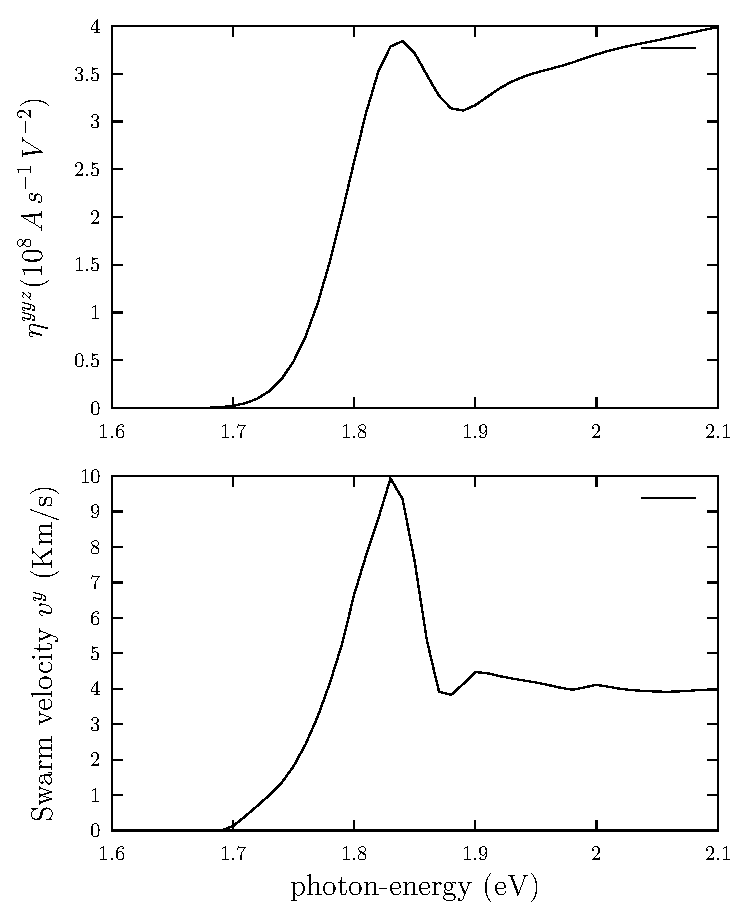
\includegraphics[scale=.7]{plots/eta-vs}
\end{center}
\caption{$\eta^{yyz}=\eta^{xxz}$ and the swarm velocity $v^y_s$ for CdSe 
  calcuated with spin-orbit interaction. 
}
\label{fig:eta-vs}
\end{figure}

\begin{figure}[t]
\begin{center}
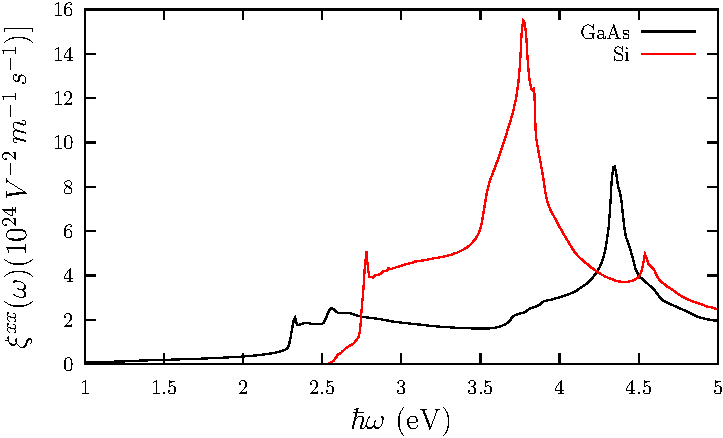
\includegraphics[scale=.7]{plots/xi}
\end{center}
\caption{$\xi^{xx}=\xi^{yy}=\xi^{zz}$ for Si and GaAs 
  calcuated with spin-orbit interaction. 
}
\label{fig:xi}
\end{figure}
\begin{figure}[h]
\begin{center}
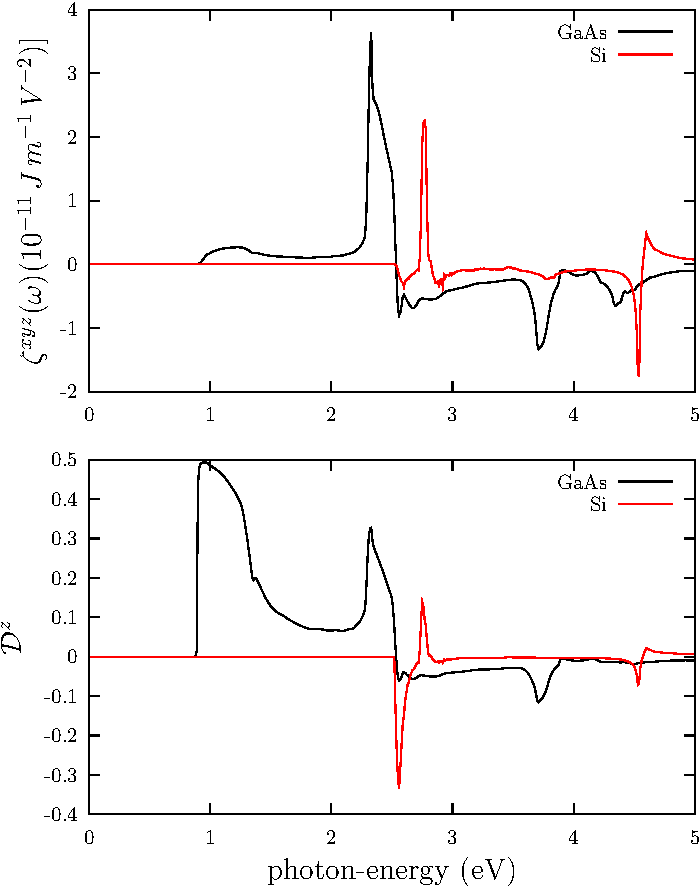
\includegraphics[scale=.5]{plots/zeta}
\end{center}
\caption{$\zeta^{xyz}$ and $\cald^z$ for Si and GaAs. 
}
\label{fig:zeta}
\end{figure}


\section{Wien2k}
In general you can use a all electron (wien2k) or pseudopotential 
(abinit) codes in order to calculate 
the first and second order response, you can follow the next seteps to 
achive the result using wien2k code. 
Now from here the user is going to be: usrname but it could be anybody, then 
take care of this. 
\begin{itemize}
\item /home/usrname/temporal/GAAS/wien2k-GAAS/GAAS >cd ~/temporal/
\item /home/usrname/temporal >~/\$TINIBA/wien2k/creatingTree.sh GAAS
\item /home/\$USER/\$TINIBA/wien2k/\textcolor{darkgreen}{creatingTree.sh} 
\begin{verbatim}
$HOME/temporal >~/\$TINIBA/wien2k/creatingTree.sh GAAS
	=====================
	=====================
	Making tree to run abinis and wien2k 
	$HOME/temporal/GAAS/abinit-GAAS/GAAS
	$HOME/temporal/GAAS/wien2k-GAAS/GAAS
	=====================

	=====================
$HOME/temporal/GAAS
   +---abinit-GAAS
      |   +---GAAS
   +---wien2k-GAAS
      |   +---GAAS
	=====================
\end{verbatim}

\item 
 \begin{verbatim}
 $HOME/temporal >cd $HOME/temporal/GAAS/wien2k-GAAS/GAAS
$HOME/temporal/GAAS/wien2k-GAAS/GAAS >
 \end{verbatim}
\item /home/\$USER/\$TINIBA/wien2k/\textcolor{darkgreen}{wien2k.sh} 
\begin{verbatim}
Usage: 
	$HOME/\$TINIBA/wien2k/wien2k.sh  [option-0]  [option-1] 
	[option-0] = scf    -run ONLY scf 
	[option-0] = klist  -generate rklist
	[option-0] = run    -run ONLY momentum and energy  matrix elements 
	[option-0] = help   -example files for si bulk 
	[option-0] = clean_lapw -remove unnecessary files 
	[option-0] = whatneed   -what files I need  
	[option-1] = 0.001      -energy convercence LIMIT (0.0001 Ry)
	===================
	$HOME/\$TINIBA/wien2k/wien2k.sh scf 0.001
	$HOME/\$TINIBA/wien2k/wien2k.sh klist
	$HOME/\$TINIBA/wien2k/wien2k.sh run 
	$HOME/\$TINIBA/wien2k/wien2k.sh clean_lapw
	$HOME/\$TINIBA/wien2k/wien2k.sh help
	Stoping right now...  wien2k.sh
\end{verbatim}



 
\end{itemize}
\section{Refinement over k-points}
If you want to refine the density of k-points over one window of energy 
you can follow this script 
\begin{itemize}
 \item /home/\$USER/\$TINIBA/\textcolor{darkgreen}{refine.sh} 
\begin{verbatim}
	Usage:
	$HOME/\$TINIBA/refine.sh abinit first
	$HOME/\$TINIBA/refine.sh abinit refine noscissors
	$HOME/\$TINIBA/refine.sh abinit refine scissors
	Stoping right now...
	$HOME/\$TINIBA/refine.sh
	I need input Args
\end{verbatim}

\end{itemize}


\section{The GW method and Bethe-Salpeter Equation}
to be done 
%\subsection{Why we have to use GW and BSE}


\section{Surfaces }
\emph{God made solids ...\\
      but surfaces were the work of the devil}, W. Pauli\\                                  
%The optics at surfaces 



\section{Contributors}
This list of contributors is not completee, if there are others let us know
\begin{itemize}
\item Bernardo Mendoza
\item Sean M. Anderson
\item JL Cabellos
\item Tonatiuh Rangel
\item Cuahutemoc Salzar
\item Norberto Arzate
%\item John Sipe
\item Fred Nastos  
\end{itemize}

to be continued$\ldots$

LAST MODIFICATION: by BMS on \date{\today }

\appendix

\section{Extras: gnuplot and Compilation}

\subsection{gnuplot}

Nice trick to plot columns from different files for the same plot

\verb=> p '< paste file1 file2 ...' u #c-file1:#c-file2 w l=\\\\
where \verb=fileN= is the N-th file and 
\verb=#c-fileN= is the number of the column of \verb=fileN= to be plotted. 



\subsection{Compilation}

\begin{enumerate}
%
\item Compiling IBZ: executable \verb=ibz.medusa= or \verb=ibz.quad=
\begin{itemize}
\item[XEON:] \verb=$HOME/tiniba/verN.M/src_ibz> make clean -f Makefile_xeon= 
\verb=$HOME/tiniba/verN.M/src_ibz> make -f Makefile_xeon= 
\item[QUAD:]\verb=ssh quad01=

\verb=$HOME/tiniba/verN.M/src_ibz> make clean -f Makefile_quad= 
\verb=$HOME/tiniba/verN.M/src_ibz> make -f Makefile_quad= 
\end{itemize}
%
\item Compiling matrix elements: executable \verb=rpmns.itanium= or
  \verb=rpmns.quad= or \verb=rpmns.xeon=
\begin{itemize}
\item \verb=$TINIBA/verN.M/matrix_elements/ver3.0> compilerRPMNS.sh=\\
Follow instructions to compile in the three plataforms.
\end{itemize}
%
\item Old way to calculate Second Order Response (SHG)
 
Here you must to run \textcolor{darkgreen}{responseSHG.sh} with option number 21 and 22 for lenght
 gauge formalism and 64 and 65 for velocity gauge formalism and you must provide the LDA band gap 
 in order to calcuate zero scissors correction and you must provide experimental band gap in order to 
calculate the SHG with scissors correction. The typical value of semar is 0.15 eV, in the case of GaAs 
 the tensor componet different of zero is xzy.
when you finish with the \textcolor{darkgreen}{glue.sh} script, if everething is ok, you get  a file
that contains in the first row energy in eV,  the second one the real part of $1\;\omega$ contribution of lenght, 
the third one the imaginary part of $1\;\omega$ contribution of lenght,  
the 4 one the real part of $2\;\omega$ contribution of lenght, 
the 5 one the imaginary part of $2\;\omega$ contribution of lenght, and the others four rows (6-9)
contains the SHG for velocity formalism. (6=Re,$1\;\omega$), (7=Im,$1\;\omega$), (8=Re,$2\;\omega$) and 
(9=Im,$2\;\omega$)\\
If you want to plot the $|\chi_2^{xyz}|$ for lenght gauge formalism in the case of GaAs, the typical line text in gnuplot is 
\begin{verbatim}
p 'shg1l_shg2l_shg1t_shg2t_xxz_sm_0-150_3876_10-
nospin_32_N_0-849_0-0d0_0-0d0L_0-0d0t_SRC_response'  
u 1:(sqrt(($2+$4)**2+($3+$5)**2)) smooth csplines title '$\chi^2_{xyz}$'
w l lw 2
\end{verbatim}

   
\begin{itemize}
\item \verb=$HOME/$TINIBA/SRC_response/=\textcolor{darkgreen}{responseSHG.sh} 
\item \verb=$HOME/$TINIBA/SRC_response/all/=\textcolor{darkgreen}{doNuevoSmearingt$_{-}$juniot$_{-}$14t$_{-}$2010.sh} 
\item \verb=$HOME/$TINIBA/1response/=\textcolor{darkgreen}{glue.sh} 
\end{itemize}

\end{enumerate}

\begin{figure}[t]
\begin{center}
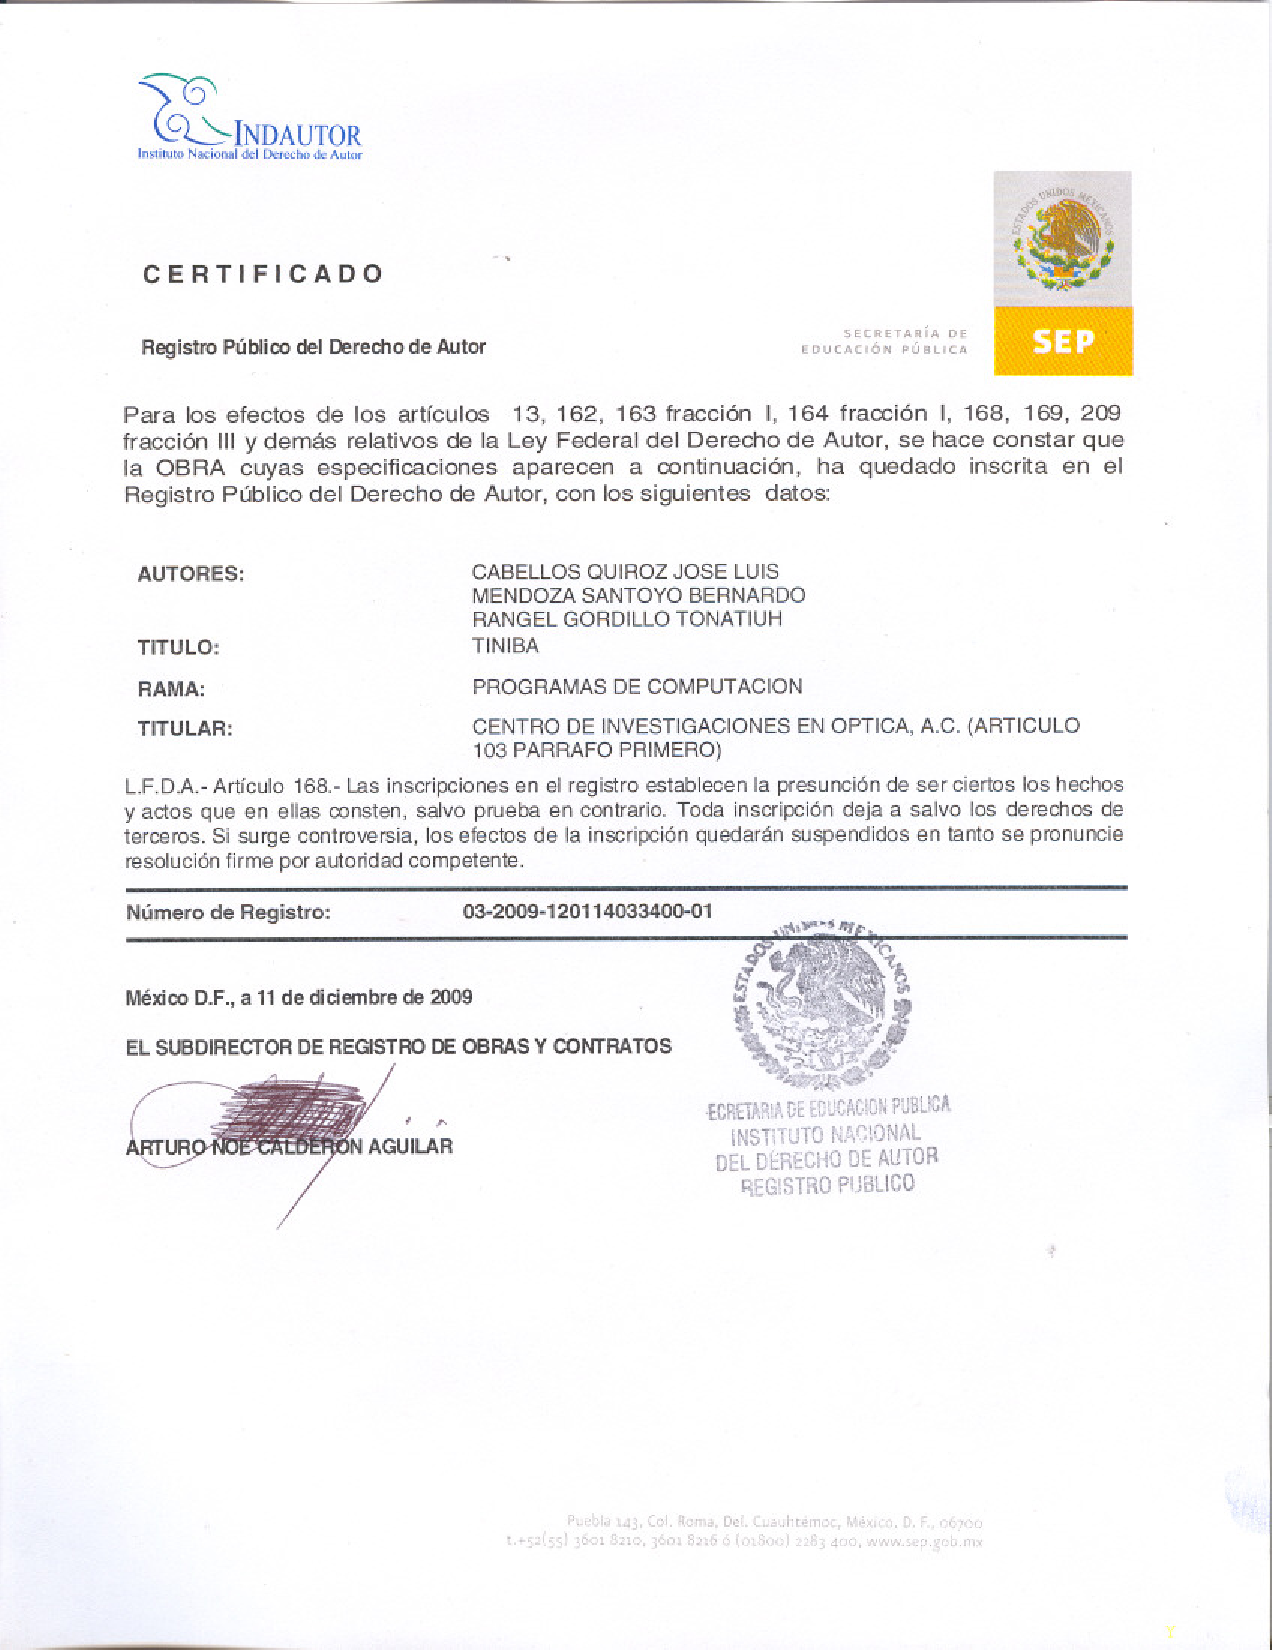
\includegraphics[scale=0.6]{CERTIFICADO-INDAUTOR-TINIBA1}
\end{center}
\caption{INDAUTOR Certificate of TINIBA$^{\reg}$ 
}
\label{inpi}
\end{figure}

\end{document}                          % The required last line

%%%%% usless for DSP below

\item  Using \verb=chose_layers.sh= select the following layers: 
\begin{enumerate}
\item front-layer $\to\ell=$\verb=1=
\item back-layer $\to\ell=$\verb=N=
\item middle-layer $\to\ell=$\verb=middle=
\item half-slab $\to\ell=$\verb=half-slab= (by default is the {\it
   front} half-slab)\\
then run \verb=run_tiniba.sh= with option \verb=-N 4=
\item[and]
\item full-slab: 
run \verb=run_tiniba.sh= with option \verb=-N 0=
\end{enumerate}

\item Then, the different responses are given by:
\begin{eqnarray}\label{surfj}
\tilde\chi^{\mathrm{front-surface}}
&=&
\chi^{\mathrm{half-slab}}-\ell_B
\chi^{\mathrm{middle}}\nonumber
\\
\tilde\chi^{\mathrm{back-surface}}
&=&
\underbrace{\left(\chi^{\mathrm{full-slab}}-
\chi^{\mathrm{half-slab}}
\right)}_{\mathrm{back-surface}}
-\ell_B
\chi^{\mathrm{middle}}
\nonumber
,
\end{eqnarray}   
with $\ell_B$ the integer value of the middle layer. Also
$\tilde\chi^i=\left(A/\gO\right)\chi^j$ 
and
$\chi^j$ is $\zeta^{j,\rma\rmb\rmc}$ or
$\xi^{j,\rmb\rmc}$, with $i=$front-surface or back-surface and
$j=$full-slab, half-slab or middle.
%%%%% usless for DSP above

Tiniba is a suit of scripts to run and calculate optical properties of
crystalline semiconductors by parallelizing the computation of the
different quantities involved in the procedure.     

